% CHIL 2027 submission draft. The official CHIL 2027 Overleaf template is due Nov 15, 2026;
% until then this uses the PMLR jmlr class that CHIL proceedings are published in.
% Long-form version (thesis): main.tex. Shared: refs.bib, figures/.
\documentclass[wcp]{jmlr}
\usepackage{booktabs,multirow,adjustbox}
\newcommand{\todo}[1]{\textcolor{red}{[TODO: #1]}}
\newcommand{\passk}[1]{\mathrm{pass@}#1}
\jmlrvolume{}
\jmlryear{2027}
\jmlrworkshop{Conference on Health, Inference, and Learning (CHIL) 2027}
\title[Sampled or Stated?]{Sampled or Stated? A Clinical Measurement Study of How Post-Training Changes a Language Model's Differential Diagnosis}
\author{\Name{Anonymous Authors}\\ \addr Anonymous Institution}

\begin{document}
\maketitle

\begin{abstract}
A language model's differential diagnosis can be read from the ranked list it states in one answer or from the spread of its answers over repeated samples; pass@$k$, self-consistency and sampling-based uncertainty use the second. Instruction-tuned models are known to sample poorly from distributions they can describe.
In a clinical measurement study, we test what this means for differential diagnosis, with base/post-trained pairs from two open families at 7--32B (Qwen2.5-7B and -32B, Qwen3-8B, and every released stage of OLMo~3 7B and OLMo~3.1 32B) and three medical models, using 32 samples per case on DDXPlus, whose synthetic patients carry a rule-based reference differential, and on real rare-disease cases from Phenopacket Store.
Post-training narrows the sampled answers to 1.3--3.6 distinct top answers per 32 samples, against 3.8--8.2, and in five of eight settings leaves them farther from the reference than a guesser that ignores the patient.
The stated list moves the other way, closer to the reference even with the true diagnosis removed, for Qwen at 7--32B under zero- and few-shot prompts and for OLMo~3.1 32B under the zero-shot prompt only, but not for OLMo~3 7B; yet post-trained lists name 4--8 of the 17 severe conditions less often.
Majority voting stops helping and agreement between samples becomes a weaker error signal; a two-feature combination of agreement and stated probability, fitted on 100 labeled cases, beats either signal alone. These patterns replicate in a third family (Mistral-7B, prompted with worked examples), and the mean of five base-model lists is about as close to the reference as one post-trained list; Qwen3-8B's thinking mode instead restores the sampled answers.
On real cases the shifts appear without a crossover. Which post-training stage narrows the samples most depends on the recipe.
Evaluations of diagnostic breadth should say which readout they use.
\end{abstract}

\paragraph{Data and Code Availability.}
All data are public: DDXPlus~\citep{fansi2022ddxplus} (synthetic patients) and Phenopacket Store v0.1.27~\citep{danis2025phenopacketstore} (cases from published literature). All models are public checkpoints (Table~\ref{tab:models}). Prompts and an example vignette are in Appendix~\ref{app:prompts}; code and sampled outputs will be released with the camera-ready version.

\paragraph{Institutional Review Board (IRB).}
This work uses only public synthetic or previously published, de-identified data and involves no human subjects, so it did not require IRB review.

%=====================================================================
\section{Introduction}\label{pg:mainstart}
Clinicians reason over a differential diagnosis, a ranked set of conditions consistent with the presentation, and the conditions they keep in view determine which tests are ordered and which dangerous possibilities are ruled out.
A language model's differential can be read in two ways: from the list it states in one answer, or from the distribution of its answers over repeated samples.
Much current practice uses the second. Pass@$k$, self-consistency voting~\citep{wang2023selfconsistency} and sampling-based uncertainty such as semantic entropy~\citep{farquhar2024semanticentropy} draw on repeated samples, and so does the evidence that reinforcement learning sharpens models, which win at $\passk{1}$ while their base models solve more problems given many samples~\citep{yue2025rlboundary,wu2025invisibleleash,oh2026sharpeningtax}.
The two readouts agree for a model that samples from the distribution it states. Instruction-tuned models do not: they verbalize distributions they fail to sample from~\citep{meister2025distributional,zhang2025verbalized,jang2026cannotsample}, and one aligned answer can cover what many base-model samples spread out~\citep{lake2025overton}.
We measure what this means for differential diagnosis, where a reference differential and a true diagnosis are available for every case. This is a replication and extension of that work in a clinical setting, not a new phenomenon.

The design holds the pretrained weights fixed and varies only the post-training: base/instruct pairs for Qwen2.5-7B, Qwen3-8B and Qwen2.5-32B; every released stage (SFT, DPO, RL) of OLMo~3 7B~\citep{olmo2025olmo3} and OLMo~3.1 32B, plus a 7B checkpoint trained with RL directly from the base; and three medical models fine-tuned from Qwen2.5-7B-Instruct. As checks, we add Mistral-7B v0.3 with a few-shot prompt and Qwen3-8B with its thinking mode on.
On DDXPlus~\citep{fansi2022ddxplus}, which ships a reference differential for every synthetic patient, we score both readouts against that reference. On real rare-disease cases we score accuracy, voting and uncertainty~\citep[Phenopacket Store;][]{danis2025phenopacketstore}.
Our measurements:
\begin{itemize}
\item \textbf{Sampled answers narrow} after post-training at 7--32B, often to below a patient-blind guesser's fit to the reference, and the stage that narrows them most depends on the recipe; a reasoning mode largely restores them (\S\ref{sec:sampled}).
\item \textbf{Stated lists move closer to the reference}, even with the true diagnosis removed and by DDXPlus's own set metric, for Qwen under zero- and few-shot prompts (for OLMo~3.1 32B only zero-shot), though they name specific severe conditions, such as acute pulmonary edema and NSTEMI, less often (\S\ref{sec:stated}).
\item \textbf{Sampling-based methods lose value.} Majority voting stops helping and agreement weakens as an error signal; combining it with the stated probability on 100 labeled cases works better than either (\S\ref{sec:consequences}).
\item \textbf{On real rare-disease cases} the same shifts appear but stop short of a crossover (\S\ref{sec:medrare}).
\end{itemize}

%=====================================================================
\section{Related work}
\paragraph{Post-training and the sampled distribution.}
RL with verifiable rewards improves $\passk{1}$ while base models win at large $k$ on math and code~\citep{yue2025rlboundary}, reweighting solutions already in the base model's support~\citep{wu2025invisibleleash}; a ``sharpening tax'' appears across 14 base/post-trained pairs on agentic tasks~\citep{oh2026sharpeningtax}, though RL can expand the boundary in domains under-represented in pretraining~\citep{cheng2025guru}. In medicine, the one pass@$k$ analysis we know of studies vision-language models~\citep{jeddi2026medvlmrl}. Instruction tuning and RLHF reduce output diversity~\citep{kirk2024rlhfdiversity,west2025basemodels,jiang2025hivemind,murthy2025onefish}, more so with scale for SFT~\citep{springer2026annotations}; \citet{liu2026alignmenttax} place the collapse at DPO in a Zephyr ablation, while \citet{jang2026cannotsample} find it growing at each OLMo-2 stage.

\paragraph{Stated versus sampled distributions.}
Models asked to verbalize a distribution match it better than their samples do, on opinion surveys~\citep{meister2025distributional} and on synthetic and survey targets~\citep{jang2026cannotsample}. Verbalized sampling keeps most of the base model's diversity through Tülu~3's SFT, DPO and RLVR checkpoints while direct sampling collapses~\citep{zhang2025verbalized}, and aligned answers aggregate content that base models spread across samples~\citep{lake2025overton}. Our stated readout is the verbalized top-$k$ elicitation of \citet{tian2023justask}, who show that RLHF models' verbalized confidence is better calibrated than their token probabilities. For error detection, sample consistency usually beats verbalized confidence and hybrids beat both~\citep{xiong2024express,lyu2024consistency}, including for medical diagnosis~\citep{savage2025uncertainty,ren2026medconf}, and aligned models' samples can collapse enough to leave sampling-based uncertainty without signal~\citep{liu2026alignmenttax}. We add a clinical task with a reference differential and a true diagnosis, two pipelines at 7--32B, and the consequences for aggregation and uncertainty.

\paragraph{Medical models and differential diagnosis.}
LLMs have been evaluated as differential-diagnosis aids on clinicopathological cases~\citep{kanjee2023jama,mcduff2025ddx}. Medical post-training recipes include verifier-guided SFT and PPO~\citep{chen2024huatuogpto1}, rule-based RL~\citep{liu2025alphamed} and reasoning distillation~\citep{huang2025m1}; RL and reward models tend to favor confident answers~\citep{leng2025taming,damani2025rlcr,mei2025reasoninguncertainty}. DDXPlus was built for diagnosis systems trained on differentials~\citep{fansi2022casande} and scores predicted against reference differentials as sets (recall, precision, F1); H-DDx proposes hierarchical F1 over ICD-10 instead of top-$k$ accuracy~\citep{h-ddx2025}, and MEDDxAgent studies interactive diagnosis on it~\citep{rose2025meddxagent}. \citet{puri2026beyondmode} show on DDXPlus with Qwen3-8B that single-answer RL collapses sampled answers and train models to output several answers per completion, which then cover more of the gold differential. We compare stated and sampled differentials against the reference \emph{distribution} across public post-training pipelines.

%=====================================================================
\section{Setup}\label{sec:setup}
\paragraph{Tasks.}
\textbf{DDXPlus}~\citep{fansi2022ddxplus}: synthetic patients from a rule-based medical knowledge base, each with a true pathology and a reference differential, the engine's posterior over 49 conditions. We use 980 test patients (20 per condition) rendered by template as questionnaire-style vignettes without exam or test results (example in Appendix~\ref{app:prompts}). The prompt lists the 49 conditions and asks for the five most likely, with probabilities, as JSON, so this is a closed-set task.
\textbf{Phenopacket Store}~\citep{danis2025phenopacketstore}: 1,401 published rare-disease cases covering 749 diseases (at most two per disease), rendered as phenotype vignettes with an open-ended differential; names are graded against the case's diagnosis via Mondo as exact, related (a specific ancestor group or subtype) or wrong (Appendix~\ref{app:prompts}).

\paragraph{Models.}
Qwen2.5-7B, Qwen3-8B and Qwen2.5-32B, each with its official post-trained version; OLMo-3-1025-7B and OLMo-3-1125-32B with the SFT, DPO and final RLVR (Instruct) checkpoints of OLMo~3 7B and OLMo~3.1 32B, plus OLMo-3-7B-RL-Zero-General, trained with RL from the 7B base; and AlphaMed (rule-based RL), HuatuoGPT-o1 (SFT then PPO) and m1 (SFT distillation), all fine-tuned from Qwen2.5-7B-Instruct (Table~\ref{tab:models}).

\paragraph{Sampling.}
32 samples per case with vLLM, at $T{=}0.7$ (top-$p$ 0.95) and, for the 7--8B models, $T{=}1$ (top-$p$ 1), each model with its own chat template (OLMo base models get their SFT checkpoint's), the same prompt, and Qwen3's thinking mode off. A sample's \emph{top answer} is valid if it is one of the 49 conditions, and its \emph{list} is valid if it names at least one; invalid answers count as wrong. They affect mainly base models (up to 47\% of samples), so base-model coverage is a lower bound (Appendix~\ref{sec:robust}).

\paragraph{Two readouts.}
The \emph{sampled} readout is the distribution of top answers over a case's samples. We report $\passk{k}$~\citep{chen2021codex}, the number of distinct top answers, the reference mass they cover (coverage@32), and total-variation distance (TV) of their empirical distribution to the reference.
The \emph{stated} readout is one sample's list, with its stated probabilities renormalized over the conditions it names (uniform if missing), averaged over valid samples. We report its TV to the reference, its TV after removing the true pathology from both list and reference, DDXPlus's set F1 against the reference's support (DDF1), the reference mass it names, and whether it names each severe condition (DDXPlus severity 1--2, the dataset's label rather than a clinical consensus list) that the reference weights at least 0.1. Since a list's TV is at least one minus the mass it names, these are not independent.
The \emph{single-call answer} is the top answer of a model's first valid sample. Intervals are 95\% percentile intervals from a paired case bootstrap, computed on unrounded values; AUROCs use average ranks for ties. The headline base-vs-post differences are also tested with a bootstrap that resamples the 49 true-pathology clusters, with Holm correction over 112 tests (Appendix~\ref{app:clustered}); we say where a result does not survive it.

%=====================================================================
\section{Results}
\subsection{Post-training narrows the sampled answers}\label{sec:sampled}
Table~\ref{tab:sampled} compares each base model with its post-trained versions.
At 7--8B the post-trained Qwen model is far better on its first answer ($+12.6$ to $+27.5$ points), but its pass@$k$ curve crosses the base model's at $k{\approx}4$--8, and at $k{=}32$ the base model leads by 9.7--14.6 points (Figure~\ref{fig:passk} in Appendix~\ref{sec:general}); these losses survive clustering and correction. At 32B the losses are smaller and do not: Qwen2.5-32B-Instruct gains 10.4 points at $k{=}1$ and loses 4.9 $[2.8,7.1]$ at $k{=}32$, OLMo~3.1 32B Instruct loses 4.0 $[2.0,5.9]$. With three worked examples in every prompt, base models answer validly and both 32B losses grow, to 15.2 and 19.1 points, and survive correction (Appendix~\ref{sec:fewshot}). Mistral-7B v0.3, prompted with the same examples, shows the same crossing ($-14.5$ points at $k{=}32$), whereas Qwen3-8B with its thinking mode on beats its base model at $k{=}32$ (0.815 against 0.732; Appendices~\ref{sec:mistral} and~\ref{sec:thinking}).
The narrowing itself is robust: post-trained models give 1.3--3.6 distinct top answers per 32 samples, against 3.8--8.2, and cover less of the reference mass. Coverage@32 favors spreading answers, though: a guesser drawing uniformly from the 49 conditions covers 0.48 and one drawing from the average reference differential 0.56, more than any model. By TV, which also rewards concentrating on the right conditions, base models' samples beat that patient-blind guesser (0.71--0.76 against 0.77), while five of the eight post-trained settings fall behind it (0.78--0.85).
Which stage narrows the samples most depends on the recipe. In OLMo~3 7B, distinct answers fall from 4.93 to 4.01 after SFT, 3.30 after DPO and 2.37 after RLVR, and the RLVR step alone costs 19.1 $[16.3,21.8]$ points of $\passk{32}$ against the DPO model. In OLMo~3.1 32B, SFT costs most (12.1 $[9.9,14.4]$ points), DPO recovers most of it, and the RLVR step costs 2.8 $[1.1,4.3]$ (Appendix~\ref{sec:big32}). RL-Zero, trained with RL from the 7B base, narrows less; at $T{=}1$ it shows no detectable loss of $\passk{32}$ ($-1.8$ $[-4.5,+0.8]$; Appendix~\ref{sec:stages}).
Severe conditions also become rarer among the sampled top answers, but even base models consider them less often than the patient-blind guesser (Appendix~\ref{sec:collapse}), so we assess them on the stated list.

\begin{table}[t]
\centering\small
\begin{adjustbox}{max width=\linewidth}
\begin{tabular}{llcccccc}
\toprule
 & & \multicolumn{4}{c}{Sampled top answers} & \multicolumn{2}{c}{Drawn from stated lists} \\
Comparison & Model & pass@1 & pass@32 & Distinct & Cov@32 & pass@32 & Distinct \\
\midrule
Qwen3-8B, $T{=}0.7$ & base & 0.388 & \textbf{0.730} & \textbf{3.76} & \textbf{0.322} & 0.780 & 7.79 \\
 & post-trained & \textbf{0.558} & 0.607 & 1.27 & 0.217 & \textbf{0.811} & 4.96 \\
Qwen3-8B, $T{=}1$ & base & 0.282 & \textbf{0.789} & \textbf{6.60} & \textbf{0.407} & \textbf{0.832} & 9.82 \\
 & post-trained & \textbf{0.556} & 0.643 & 1.53 & 0.236 & 0.820 & 5.40 \\
Qwen2.5-7B, $T{=}0.7$ & base & 0.352 & \textbf{0.695} & \textbf{4.91} & \textbf{0.335} & 0.772 & 10.68 \\
 & instruct & \textbf{0.478} & 0.598 & 1.82 & 0.239 & \textbf{0.802} & 6.81 \\
Qwen2.5-7B, $T{=}1$ & base & 0.239 & \textbf{0.766} & \textbf{8.23} & \textbf{0.422} & 0.785 & 12.44 \\
 & instruct & \textbf{0.464} & 0.663 & 2.65 & 0.290 & \textbf{0.827} & 7.76 \\
Qwen2.5-32B, $T{=}0.7$ & base & 0.500 & \textbf{0.795} & \textbf{3.78} & \textbf{0.352} & 0.850 & 8.79 \\
 & instruct & \textbf{0.604} & 0.746 & 1.68 & 0.276 & \textbf{0.880} & 6.49 \\
\midrule
OLMo~3 7B, $T{=}0.7$ & base & 0.178 & \textbf{0.705} & \textbf{4.93} & \textbf{0.351} & \textbf{0.719} & 8.66 \\
 & SFT & 0.222 & 0.559 & 4.01 & 0.257 & 0.618 & 7.18 \\
 & SFT+DPO & \textbf{0.324} & 0.613 & 3.30 & 0.272 & 0.702 & 6.88 \\
 & SFT+DPO+RLVR & 0.266 & 0.422 & 2.37 & 0.195 & 0.577 & 5.65 \\
 & RL-Zero (from base) & 0.295 & 0.572 & 4.06 & 0.286 & 0.701 & 9.66 \\
\midrule
OLMo~3.1 32B, $T{=}0.7$ & base & 0.326 & \textbf{0.796} & \textbf{4.32} & \textbf{0.347} & 0.839 & 8.11 \\
 & SFT & 0.461 & 0.674 & 2.94 & 0.265 & 0.759 & 7.94 \\
 & SFT+DPO & \textbf{0.584} & 0.784 & 2.29 & 0.293 & \textbf{0.868} & 6.64 \\
 & SFT+DPO+RLVR & 0.560 & 0.756 & 2.15 & 0.283 & 0.853 & 6.75 \\
\midrule
Chance & uniform guesser & 0.020 & 0.48 & 23.7 & 0.48 & & \\
 & reference-prior guesser & --- & 0.44 & 21.9 & 0.56 & & \\
\bottomrule
\end{tabular}
\end{adjustbox}
\caption{Sampled readout on DDXPlus (980 cases, 32 samples). Distinct: distinct top answers per case; Cov@32: reference mass they cover. \emph{Drawn from stated lists}: each sample's top answer replaced by a draw from its own stated list. Bold: better model of each pair (OLMo: of the block). Invalid answers count as wrong, which mostly penalizes base models. Chance: guessers that ignore the patient, drawing uniformly from the 49 conditions or from the reference differential averaged over test cases.}
\label{tab:sampled}
\end{table}

\subsection{Stated lists move closer to the reference}\label{sec:stated}
Post-training moves the stated list the other way (Figure~\ref{fig:stated}a, Table~\ref{tab:stated}). For every Qwen model and OLMo~3.1 32B, the post-trained model's single list is closer to the reference than its base model's (TV $-0.043$ to $-0.088$ for Qwen, $-0.045$ for OLMo~3.1 32B), while its samples move away. Three controls make this more than the side effect of higher accuracy or longer lists. With the true pathology removed from both list and reference, the post-trained list is still closer ($-0.018$ to $-0.056$; for Qwen3-8B at $T{=}0.7$ the corrected $p$ is 0.05). By DDXPlus's own set F1 it improves by 0.040--0.083. A fixed patient-blind list, the top five of the average reference differential, scores TV 0.794; every model's list beats it except OLMo~3 7B's. With three worked examples in every prompt, the Qwen gains persist or grow (TV $-0.057$ to $-0.087$; $-0.055$ to $-0.073$ without the true pathology), but OLMo~3.1 32B's list keeps only its higher reference mass ($+0.047$), with TV, TV without the true pathology and DDF1 no longer significant (Appendix~\ref{sec:fewshot}). Averaging calls narrows the gap: the mean of five base-model lists is about as close to the reference as one post-trained list (Qwen3-8B 0.699 against 0.701), so direct-answer post-training mostly packs into one call what the base model spreads across calls; only Qwen3-8B's thinking mode beats averaged base lists (Appendix~\ref{sec:aggregate}).
OLMo~3 7B is the exception: its five-item Instruct lists are no closer to the reference than its base model's, with or without the true pathology, and are worse than the patient-blind list. Asked for a probability on every condition, its stated distribution does move closer ($-0.032$; Appendix~\ref{sec:fullprompt}), while the Qwen pairs reproduce their five-item results.
The average hides losses that matter clinically. Post-trained lists name severe conditions that the reference weights at least 0.1 more often for Qwen ($+9.0$ to $+13.8$ points), but for each pair 4--8 of the 17 severe conditions are named less often wherever the reference gives them any weight, among them acute pulmonary edema (Qwen2.5-32B 0.63 $\rightarrow$ 0.44, OLMo~3 7B 0.56 $\rightarrow$ 0.31), NSTEMI/STEMI (OLMo~3.1 32B 0.49 $\rightarrow$ 0.36), stable angina (Qwen2.5-7B 0.25 $\rightarrow$ 0.08) and pulmonary embolism (OLMo~3.1 32B 0.39 $\rightarrow$ 0.31) (Appendix~\ref{sec:statedchecks}). Whether lists name more unwarranted severe conditions (reference weight below 0.1) varies by model, from 0.22 fewer per list (OLMo~3.1 32B) to 0.35 more (OLMo~3 7B).
Drawing each top answer from the sample's own stated list raises $\passk{32}$ for every model (Table~\ref{tab:sampled}); post-trained lists reach higher than their base model's lists in five of seven comparisons (not Qwen3-8B at $T{=}1$ or OLMo~3 7B). In absolute terms every model stays far from the reference: one list names 0.26--0.42 of its mass, against 0.74 for the reference's own top five.

\begin{figure}[t]
\centering
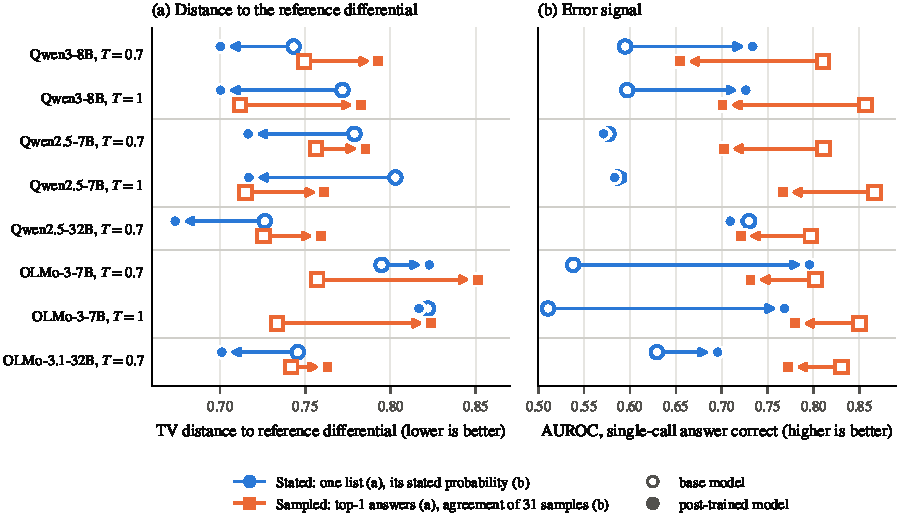
\includegraphics[width=\linewidth]{figures/fig_stated_sampled.pdf}
\caption{Base (hollow) $\rightarrow$ post-trained (filled) on DDXPlus (980 cases; OLMo: base $\rightarrow$ final Instruct; 32B models at $T{=}0.7$). (a) TV distance to the reference differential of one stated list (blue circles) and of the sampled top answers (orange squares): post-training moves the list toward the reference and the samples away from it, except for OLMo~3 7B's five-item lists. (b) AUROC for the single-call answer being correct, of its stated probability (blue) and of agreement across 31 further samples (orange).}
\label{fig:stated}
\end{figure}

\begin{table}[t]
\centering\small
\begin{adjustbox}{max width=\linewidth}
\begin{tabular}{llcccccc}
\toprule
 & & \multicolumn{3}{c}{TV to reference$\downarrow$} & & Reference & Severe \\
Comparison ($T{=}0.7$) & Model & One list & Samples & List w/o gold & DDF1 & mass named & named \\
\midrule
Qwen3-8B & base & 0.743 & \textbf{0.749} & 0.833 & 0.276 & 0.335 & 0.347 \\
 & post-trained & \textbf{0.700} & 0.793 & \textbf{0.815} & \textbf{0.318} & \textbf{0.396} & \textbf{0.437} \\
Qwen2.5-7B & base & 0.779 & \textbf{0.756} & 0.856 & 0.245 & 0.291 & 0.345 \\
 & instruct & \textbf{0.716} & 0.785 & \textbf{0.816} & \textbf{0.307} & \textbf{0.364} & \textbf{0.440} \\
Qwen2.5-32B & base & 0.726 & \textbf{0.726} & 0.830 & 0.282 & 0.352 & 0.382 \\
 & instruct & \textbf{0.674} & 0.759 & \textbf{0.787} & \textbf{0.333} & \textbf{0.418} & \textbf{0.472} \\
OLMo~3 7B & base & \textbf{0.795} & \textbf{0.757} & \textbf{0.850} & \textbf{0.225} & \textbf{0.268} & 0.256 \\
 & Instruct (RLVR) & 0.823 & 0.851 & 0.884 & 0.220 & 0.257 & \textbf{0.317} \\
OLMo~3.1 32B & base & 0.746 & \textbf{0.742} & 0.835 & 0.273 & 0.335 & 0.371 \\
 & Instruct (RLVR) & \textbf{0.701} & 0.763 & \textbf{0.812} & \textbf{0.312} & \textbf{0.391} & \textbf{0.392} \\
\midrule
Chance & patient-blind & 0.794 & 0.774 & --- & 0.272 & 0.238 & 0.149 \\
Oracle & reference & 0.265 & 0.18--0.25 & --- & --- & 0.735 & 0.975 \\
\bottomrule
\end{tabular}
\end{adjustbox}
\caption{Stated vs.\ sampled readouts on DDXPlus ($T{=}0.7$, 980 cases, valid samples). \emph{One list}: one sample's stated differential (mean over samples). \emph{Samples}: empirical distribution of top answers. \emph{List w/o gold}: TV after removing the true pathology from list and reference. DDF1: set F1 of the named conditions against the reference's support. \emph{Severe named}: share of severe conditions with reference probability $\geq 0.1$ that one list names. Chance: the top five of the average reference differential as a fixed list, and 32 draws from that average as samples. The readouts have different floors (Oracle: the reference's own top five; as many reference draws as valid samples), so compare each across models; floor-corrected values are in Table~\ref{tab:robust}. Bold: better model of each pair.}
\label{tab:stated}
\end{table}

\subsection{Consequences for sampling-based methods}\label{sec:consequences}
Table~\ref{tab:consequences} asks what the gap does to two uses of repeated samples.

\paragraph{Aggregation.}
Majority voting over 32 samples (self-consistency) raises base models' accuracy by 3.4--8.4 points at $T{=}0.7$, but adds little for the final post-trained models (Qwen3-8B $+0.3$, Qwen2.5-7B-Instruct $+0.8$, OLMo-3-7B-Instruct $-0.2$, OLMo-3.1-32B-Instruct $+0.9$, all n.s.; Qwen2.5-32B-Instruct $+1.9$ $[0.5,3.5]$). Models that reason before answering still gain (HuatuoGPT-o1 $+4.8$, m1 $+3.8$, Qwen3-8B with a CoT prompt $+4.5$). Counting an invalid first sample as wrong instead of skipping it raises the base models' voting gains (5.6--18.4 points) and leaves the final post-trained models' at most 1.7. For a top-three differential, the top three of one list contains the true pathology more often than the three most frequent of 32 sampled answers for the post-trained Qwen models ($+13.7$ $[11.4,15.9]$ for Qwen3-8B, $+7.3$ for Qwen2.5-7B-Instruct, $+5.6$ for Qwen2.5-32B-Instruct), while for every base model the samples win by 7.3--13.6 points.

\paragraph{Uncertainty.}
We score each signal by how well it ranks the correctness of the single-call answer (AUROC). The stated probability needs no extra calls; \emph{agreement}, the share of other samples with the same top answer, needs 4 or 31. For base models agreement is far better (0.80--0.83 against 0.54--0.73). Post-training weakens it in every family (Qwen3-8B 0.810 $\rightarrow$ 0.655, Qwen2.5-7B 0.811 $\rightarrow$ 0.702, Qwen2.5-32B 0.797 $\rightarrow$ 0.721, OLMo~3 7B 0.802 $\rightarrow$ 0.731, OLMo~3.1 32B 0.831 $\rightarrow$ 0.772; Figure~\ref{fig:stated}b), consistent with \citet{liu2026alignmenttax}; the paired drop survives clustering and correction for every Qwen pair but not for OLMo. For Qwen3-8B and OLMo-3-7B-Instruct the stated probability is then the better signal ($+0.079$ $[0.046,0.110]$ and $+0.064$ $[0.027,0.101]$ over 32-sample agreement); for the other final models agreement stays better or ties, in line with \citet{savage2025uncertainty}. With its thinking mode on, Qwen3-8B returns to the base-model pattern (agreement 0.693 against 0.638; Appendix~\ref{sec:thinking}).

\paragraph{Which signal to use.}
Across 56 model--setting combinations (the models above at both temperatures and three prompts, our GRPO runs and a full-distribution prompt; they share weights, so we treat the results as descriptive), the stated probability's advantage over five-sample agreement tracks the share of cases whose five samples all agree (Spearman 0.75). Rather than choose, a practitioner can combine. Fitting a logistic model of correctness on the two signals with 100 labeled cases and five samples each, and evaluating on the other 880, gives a held-out AUROC of 0.753 for the 39 post-trained combinations, against 0.720 for picking the better single signal on the same 100 cases, 0.695 for always using agreement and 0.671 for always using the stated probability; it beats the single-signal pick for 35 of the 39. The cost is gold labels for 100 cases from the target population (Appendix~\ref{sec:audit}).

\paragraph{Ambiguity.}
For every model and signal, the Spearman correlation between uncertainty and the entropy of the case's reference differential lies between $-0.11$ and $+0.16$, except AlphaMed's stated probability ($+0.30$): by either readout, a model's uncertainty says almost nothing about how ambiguous a case is.

\begin{table}[t]
\centering\small
\begin{adjustbox}{max width=\linewidth}
\begin{tabular}{lcccccc}
\toprule
 & Single-call & Vote@32 & Top-3: list & \multicolumn{3}{c}{AUROC, single-call answer correct} \\
Model & accuracy & gain & $-$ 32 samples & Stated $p$ & Agree@5 & Agree@32 \\
\midrule
Qwen3-8B-Base & 0.456 & $+3.4$ & $-7.3$ & 0.595 & 0.772 & \textbf{0.810} \\
Qwen3-8B & 0.556 & $+0.3$ & $+13.7$ & \textbf{0.734} & 0.613 & 0.655 \\
Qwen3-8B (CoT prompt) & 0.648 & $+4.5$ & $+0.0$ & 0.718 & 0.725 & \textbf{0.778} \\
Qwen2.5-7B & 0.371 & $+5.2$ & $-8.9$ & 0.576 & 0.764 & \textbf{0.811} \\
Qwen2.5-7B-Instruct & 0.480 & $+0.8$ & $+7.3$ & 0.571 & 0.653 & \textbf{0.702} \\
Qwen2.5-32B & 0.510 & $+7.0$ & $-8.3$ & 0.730 & 0.759 & \textbf{0.797} \\
Qwen2.5-32B-Instruct & 0.598 & $+1.9$ & $+5.6$ & 0.709 & 0.663 & \textbf{0.721} \\
\midrule
OLMo-3 7B base & 0.291 & $+4.0$ & $-13.6$ & 0.538 & 0.761 & \textbf{0.802} \\
OLMo-3 7B SFT+DPO & 0.327 & $-0.4$ & $-7.8$ & 0.738 & 0.702 & \textbf{0.751} \\
OLMo-3-7B-Instruct & 0.267 & $-0.2$ & $+1.9$ & \textbf{0.796} & 0.668 & 0.731 \\
OLMo-3.1 32B base & 0.441 & $+8.4$ & $-13.2$ & 0.629 & 0.805 & \textbf{0.831} \\
OLMo-3.1-32B-Instruct & 0.562 & $+0.9$ & $-0.6$ & 0.696 & 0.712 & \textbf{0.772} \\
\midrule
AlphaMed-7B & 0.528 & $+0.9$ & $+0.6$ & 0.673 & 0.663 & \textbf{0.715} \\
HuatuoGPT-o1-7B & 0.532 & $+4.8$ & $-0.4$ & 0.590 & 0.715 & \textbf{0.775} \\
m1-7B & 0.495 & $+3.8$ & $-4.6$ & 0.680 & 0.736 & \textbf{0.782} \\
\bottomrule
\end{tabular}
\end{adjustbox}
\caption{Aggregation and uncertainty on DDXPlus ($T{=}0.7$, 980 cases). Single-call accuracy uses the first valid sample, so it can exceed pass@1, which counts invalid answers as wrong. Vote@32 gain: accuracy of the majority top answer over all valid samples minus single-call accuracy (points). Top-3: rate at which one list's top three contains the true pathology minus the rate for the three most frequent sampled answers (points). AUROC: stated probability of the single-call answer (no extra calls) vs.\ agreement of 4 or 31 further samples; bold marks the best signal.}
\label{tab:consequences}
\end{table}

\subsection{Real rare-disease cases and medical post-training}\label{sec:medrare}
\paragraph{Real rare-disease cases.} Phenopacket Store has no reference differential and accuracy is near the floor, so here we count an answer as correct if it is the diagnosis or a closely related Mondo class (36--130 correct single-call answers per model; Appendix~\ref{sec:phenoreadouts}). The DDXPlus shifts reappear, without a crossover. Majority voting over 32 samples helps the base models by 3.1--4.6 points but the final post-trained models by only 0.4--1.5 (Qwen3-8B $+0.4$, n.s.). Post-training weakens agreement as an error signal (Qwen3-8B 0.830 $\rightarrow$ 0.763, Qwen2.5-7B 0.845 $\rightarrow$ 0.745, OLMo~3 7B 0.814 $\rightarrow$ 0.726) and strengthens the stated probability (0.567 $\rightarrow$ 0.707, 0.598 $\rightarrow$ 0.717, 0.464 $\rightarrow$ 0.652): agreement beats the stated probability by 0.25--0.35 AUROC for the base models but by only 0.03--0.07 for the post-trained ones, a difference that remains detectable only for Qwen3-8B. On these open-ended cases the three most frequent of 32 sampled answers still contain a correct diagnosis more often than one list's top three, but the gap shrinks from 4.6--7.0 points for the base models to 2.7--3.6 for Qwen2.5-7B-Instruct and OLMo-3-7B-Instruct and to a tie for Qwen3-8B ($+0.4$, n.s.).

\paragraph{Medical models.} Medical post-training on Qwen2.5-7B-Instruct adds DDXPlus accuracy without narrowing the samples further: AlphaMed (rule-based RL) improves on its parent at every $k$ ($+3.9$ at $k{=}1$, $+8.4$ at $k{=}32$) with unchanged sampled diversity (1.87 vs.\ 1.82 distinct answers), and HuatuoGPT-o1 and m1, both trained on reasoning traces, widen the sampled differential (2.49 and 3.29). AlphaMed's checkpoint trained from the base model keeps most of the base model's diversity (3.14 distinct answers; Appendix~\ref{sec:medical}).
On Phenopacket Store every model is near the floor ($\passk{32}$ 2.5--7.0\%), but stated confidence is not: the RL-trained medical models (AlphaMed; HuatuoGPT-o1 after SFT) raise it from 0.51 for the parent to 0.67--0.69 (0.71 for AlphaMed's base-initialized checkpoint) while accuracy gains stay under 1.5 points, and every OLMo~3 7B stage states 0.73--0.84 at about 1\% accuracy. At this accuracy, ECE mostly restates confidence, so we read this as confidence rising without accuracy (Appendix~\ref{sec:rare}).

%=====================================================================
\section{Discussion and limitations}
\citet{jang2026cannotsample} show that instruction-tuned models cannot sample from distributions they can describe. We measure the same split in differential diagnosis, against a reference differential with a known true pathology, in two open pipelines at 7--32B: post-training improves the list a model states on average while narrowing the answers it samples. Evaluations that read the differential from samples (pass@$k$ at large $k$, sample diversity, self-consistency, agreement-based uncertainty) therefore report a loss that a clinician reading one answer would not see, and lose value as tools on post-trained models. These effects belong to answering directly: Qwen3-8B's thinking mode restores large-$k$ accuracy and agreement as an error signal. For error detection, combining agreement with the stated probability on a small labeled set is better than relying on either. The stated list is no free replacement: it improves only on average, about as much as averaging five base-model lists, and drops specific dangerous conditions, every model stays far from the reference, and neither readout tracks how ambiguous a case is. Which post-training stage narrows the samples most is a property of the recipe. Appendix~\ref{sec:training} adds GRPO experiments on DDXPlus showing that RL from a base model need not narrow the samples as much as general post-training.

\paragraph{Limitations.}
DDXPlus is synthetic and closed-set: its reference differential is a rule-based engine's posterior, its vignettes are questionnaires without exam or test results, its test set is class-balanced, and the prompt lists all 49 conditions, so TV and coverage are distances to a \emph{reference} posterior, not to clinical truth, and nothing here was judged by clinicians. The main analyses give base models a zero-shot chat prompt, on which they often give invalid answers (27--47\% for OLMo) that we count as wrong; a three-example re-run of the five final pairs removes these and confirms the results except OLMo~3.1 32B's list gain, but uses one temperature and one set of examples (Appendix~\ref{sec:fewshot}). We study open 7--32B models from two families, a third (Mistral-7B) only with few-shot prompts, one reasoning mode (Qwen3-8B thinking) and no frontier models, one RL-Zero checkpoint (7B, LM-judge reward on chat prompts), and the 32B models only at $T{=}0.7$. The combination of signals is validated only within DDXPlus. Phenopacket accuracy is near the floor, its grader is rule-based and not validated against clinicians, and its cases may be in pretraining data.

\label{pg:mainend}
\paragraph{Statement on AI Use.}
An AI assistant (Claude, Anthropic) was used to write and run analysis code, to draft and edit text, and to check citations. The authors designed the study, reviewed all code, results and text, and take responsibility for the content.

\bibliography{refs}

\appendix
\sloppy
\section{Prompts, vignettes and grading}\label{app:prompts}
\sloppy
\paragraph{DDXPlus.} Each patient's coded evidence is rendered by a fixed template into a vignette of the patient's answers and relevant history; we fix known mistranslations in the English evidence descriptions. An example (test case with true pathology chronic rhinosinusitis; the reference differential gives viral pharyngitis 0.17, chronic rhinosinusitis 0.16, cluster headache 0.15, acute rhinosinusitis 0.14, bronchitis 0.14, URTI 0.12):
\begin{quote}\small\ttfamily
A 13-year-old female presents for evaluation. Symptoms (patient answers): Do you have pain somewhere, related to your reason for consulting? Yes. Characterize your pain: burning. Do you feel pain somewhere? mouth, forehead, cheek(R), cheek(L), nose. How intense is the pain? (scale 0-10) 3. [\dots] Have you lost your sense of smell? Yes. Do you have nasal congestion or a clear runny nose? Yes. Do you have a cough? Yes. Relevant history and risk factors: Have you had a cold in the last 2 weeks? Yes. [\dots] Do you have polyps in your nose? Yes. [\dots]
\end{quote}
System prompt: \texttt{You are an experienced emergency and primary care physician.} The user turn is the vignette followed by: \texttt{Based on the patient's answers above, give your differential diagnosis. Choose ONLY from this list of possible conditions: [the 49 conditions, one per line]. List the 5 most likely conditions from the list, most likely first, with your probability that each is the correct diagnosis. Use the condition names exactly as written in the list. End your answer with a JSON array in exactly this format: [\{"diagnosis": "<name>", "probability": <number between 0 and 1>\}, ...]}. The full-distribution prompt (\S\ref{sec:fullprompt}) instead asks for a probability on every condition, summing to one, most likely first. The plain and CoT variants are described in \S\ref{sec:robust}. Base models receive the same chat-formatted prompt; OLMo base models use their SFT checkpoint's chat template.
\paragraph{Phenopacket Store.} The vignette lists the case's present and (up to ten) excluded HPO phenotypes with sex and age. System prompt: \texttt{You are an expert clinical geneticist and diagnostician.} Instructions: \texttt{List the 5 most likely specific diagnoses (use the specific disease or subtype name, e.g.\ 'Spastic paraplegia 7' rather than 'hereditary spastic paraplegia', when you can), most likely first, with your probability that each is the correct diagnosis}, followed by the same JSON format.
\paragraph{Grading open-ended names.} Each predicted name is mapped to Mondo by exact lookup against Mondo labels and synonyms (also trying any parenthesized abbreviation and the name without it), then by fuzzy matching (token-sort ratio $\geq 92$). It is \emph{exact} if it maps to the Mondo class of the case's OMIM diagnosis, and \emph{related} if it maps to a specific ancestor group of it (at most two is-a steps up, with at most 150 descendants) or to one of its subtypes; siblings sharing only a broad parent are wrong. The grader passes hand-written checks (e.g.\ ``Hereditary spastic paraplegia type 7 (SPG7)'' is exact for SPG7, ``Hereditary spastic paraplegia'' is related, and Turner syndrome is wrong for Jacobsen syndrome), but we did not validate it against clinician grading, so errors at the scale of the 1--2 point effects we report on this dataset are possible.

\section{Models}\label{app:models}
\begin{table}[h]
\centering\small
\begin{adjustbox}{max width=\linewidth}
\begin{tabular}{llll}
\toprule
Model & Parent & Post-training & Role \\
\midrule
Qwen2.5-7B & n/a & none (pretrained) & base \\
Qwen2.5-7B-Instruct & Qwen2.5-7B & general SFT + RLHF & instruct; medical parent \\
AlphaMed-7B~\citep{liu2025alphamed} & Qwen2.5-7B-Instruct & rule-based RL & medical \\
HuatuoGPT-o1-7B~\citep{chen2024huatuogpto1} & Qwen2.5-7B-Instruct & SFT + PPO (verifier) & medical \\
m1-7B-23K~\citep{huang2025m1} & Qwen2.5-7B-Instruct & SFT distillation & medical \\
Qwen3-8B-Base & n/a & none (pretrained) & base \\
Qwen3-8B & Qwen3-8B-Base & general post-training & instruct \\
Qwen2.5-32B & n/a & none (pretrained) & base \\
Qwen2.5-32B-Instruct & Qwen2.5-32B & general SFT + RLHF & instruct \\
\midrule
OLMo-3-1025-7B~\citep{olmo2025olmo3} & n/a & none (pretrained) & base \\
OLMo-3-7B-Instruct-SFT & OLMo-3-1025-7B & SFT & stage 1 \\
OLMo-3-7B-Instruct-DPO & OLMo-3 SFT & DPO & stage 2 \\
OLMo-3-7B-Instruct & OLMo-3 DPO & RLVR & stage 3 (instruct) \\
OLMo-3-7B-RL-Zero-General & OLMo-3-1025-7B & RL (LM judge) & RL from base \\
\midrule
OLMo-3-1125-32B & n/a & none (pretrained) & base \\
OLMo-3.1-32B-Instruct-SFT & OLMo-3-1125-32B & SFT & stage 1 \\
OLMo-3.1-32B-Instruct-DPO & OLMo-3.1 SFT & DPO & stage 2 \\
OLMo-3.1-32B-Instruct & OLMo-3.1 DPO & RLVR & stage 3 (instruct) \\
\bottomrule
\end{tabular}
\end{adjustbox}
\caption{Models studied. Each pair or family shares its pretrained weights, so differences reflect post-training. OLMo~3 and OLMo~3.1 release every stage of their instruct pipelines.}
\label{tab:models}
\end{table}


\section{The sampled differential in detail}\label{app:sampled}
\subsection{General post-training trades coverage for top-1 accuracy}\label{sec:general}
Table~\ref{tab:pairs} and Figure~\ref{fig:passk} compare each base model with its post-trained counterpart on DDXPlus.
In both families the post-trained model is much better on its first answer: +27.5 points for Qwen3 and +22.5 for Qwen2.5 at $T{=}1$ (intervals $[+25.3,+29.6]$ and $[+20.7,+24.4]$).
The advantage shrinks with $k$ and reverses: the curves cross at $k{\approx}4$--8, and at $k{=}32$ the base model leads by 14.6 points (Qwen3, $[+12.2,+17.1]$) and 10.3 points (Qwen2.5, $[+7.8,+12.8]$).
The pattern is the same at $T{=}0.7$ for Qwen3, crossing at $k{=}4$ with a base lead of 12.2 points at $k{=}32$ ($[+9.9,+14.9]$).
Unparsable base-model samples count as wrong, so these gaps are lower bounds.
Qwen2.5 at $T{=}0.7$ behaves the same way: +12.6 points at $k{=}1$ $[+10.7,+14.5]$ and a base lead of 9.7 at $k{=}32$ $[+7.3,+12.0]$.

\begin{table}[t]
\centering\small
\setlength{\tabcolsep}{4pt}
\begin{adjustbox}{max width=\linewidth}
\begin{tabular}{llcccccccc}
\toprule
Pair & Model & $\passk{1}$ & $\passk{32}$ & Distinct & Entropy & TV$\downarrow$ & Cov@32 & ECE$\downarrow$ \\
\midrule
\multirow{2}{*}{Qwen3-8B, $T{=}1$} & base & 0.282 & \textbf{0.789} & \textbf{6.60} & \textbf{1.31} & \textbf{0.712} & \textbf{0.407} & 0.214 \\
 & post-trained & \textbf{0.556} & 0.643 & 1.53 & 0.18 & 0.783 & 0.236 & \textbf{0.061} \\
\midrule
\multirow{2}{*}{Qwen2.5-7B, $T{=}1$} & base & 0.239 & \textbf{0.766} & \textbf{8.23} & \textbf{1.58} & \textbf{0.715} & \textbf{0.422} & 0.303 \\
 & instruct & \textbf{0.464} & 0.663 & 2.65 & 0.49 & 0.761 & 0.290 & \textbf{0.137} \\
\midrule
\multirow{2}{*}{Qwen3-8B, $T{=}0.7$} & base & 0.388 & \textbf{0.730} & \textbf{3.76} & \textbf{0.78} & \textbf{0.750} & \textbf{0.322} & 0.121 \\
 & post-trained & \textbf{0.558} & 0.607 & 1.27 & 0.11 & 0.793 & 0.217 & \textbf{0.063} \\
\bottomrule
\end{tabular}
\end{adjustbox}
\caption{DDXPlus, 32 samples per case (980 cases). The reference differential has mean entropy 1.87. Distinct and entropy refer to the top-1 answers across samples; Cov@32 is the share of reference probability mass covered by those answers. ECE is for the stated top-1 probability.}
\label{tab:pairs}
\end{table}

\begin{figure}[t]
\centering
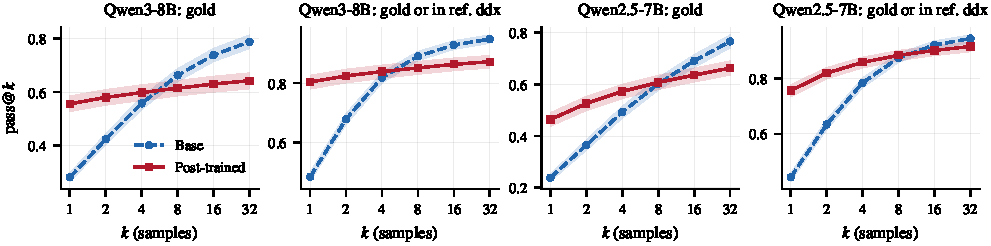
\includegraphics[width=\linewidth]{figures/fig_passk_pairs.pdf}
\caption{pass@$k$ on DDXPlus at $T{=}1$ (980 cases, 32 samples), base model (dashed) vs.\ its post-trained version (solid), with 95\% case-bootstrap bands. ``Gold'': the top-1 answer is the true pathology; ``gold or in ref.\ ddx'': it is the true pathology or appears in the reference differential. In both families the post-trained model wins at small $k$ and loses at large $k$.}
\label{fig:passk}
\end{figure}

\subsection{The sampled differential collapses, while top-1 calibration improves}\label{sec:collapse}
The gap at large $k$ reflects a collapsed \emph{sampled} differential.
Across 32 samples, the post-trained Qwen models name 1.3--2.6 distinct diagnoses per case, against 3.8--8.2 for their base models.
Their answer entropy is 0.11--0.49, against 0.78--1.58 for base models and 1.87 for the reference differential (Table~\ref{tab:pairs}).
Sampling at $T{=}1$ widens the base models' answers but barely changes the post-trained models' (Qwen3 entropy 0.11 at $T{=}0.7$, 0.18 at $T{=}1$), so the collapse lives in the model's own distribution rather than in the decoding settings.
As a result, post-trained models cover less of the reference differential: 0.24 vs.\ 0.41 of its probability mass at $k{=}32$ for Qwen3, and 0.29 vs.\ 0.42 for Qwen2.5.
Their top-1 calibration, however, is markedly better (ECE 0.06 vs.\ 0.21 and 0.14 vs.\ 0.30).
On every single-answer criterion (accuracy, small-$k$ pass@$k$, calibration), the post-trained model therefore looks strictly better, and the loss of breadth in its samples is invisible. Whether the breadth is lost from the model's stated differential as well is a separate question (\S\ref{sec:stated}).
\paragraph{Which diagnoses drop out?}
For each case and each condition that the reference differential weights at least 0.1, we ask whether the model names that condition as its top answer in at least one of its 32 samples. We call this \emph{considering} the condition.
We group the 49 conditions by DDXPlus severity (1 = most severe).
Post-training lowers consideration in every tier (Table~\ref{tab:severity}), and the severe tier (DDXPlus severity 1--2, the dataset's label rather than a clinical consensus list) is not spared. This metric needs a chance reference, though: a guesser that picks uniformly among the 49 conditions scores about 0.48 on it, and one that draws from the average reference differential 0.56--0.61, above every model, base models included. Considered@32 therefore measures the breadth of the sampled answers, not clinical judgement; we assess can't-miss conditions on the stated list instead (\S\ref{sec:statedchecks}).
For the 17 severity-1--2 conditions (e.g.\ NSTEMI/STEMI, acute pulmonary edema, anaphylaxis, pulmonary embolism, unstable angina), consideration falls from 0.45 to 0.27 for Qwen3 and from 0.51 to 0.34 for Qwen2.5 at $T{=}1$. The differences are $-18.4$ $[-20.8,-15.9]$ and $-17.0$ $[-19.7,-14.2]$ points.
Some diagnoses disappear from the top answer almost entirely.
Qwen2.5-7B-Instruct names unstable angina as its top answer in one of 107 eligible cases, where its base model does in 47\%. When unstable angina is the true pathology, $\passk{32}$ falls from 1.00 to 0.00. Stable angina (0.89 to 0.06) and myocarditis (0.41 to 0.00) follow the same pattern.
These conditions are not forgotten: they still appear lower in the listed differential (unstable angina in 50\% of eligible cases, against 95\% for the base model). The model ranks them but no longer commits to them.
At the same time, post-trained models concentrate on a few salient ``attractor'' diagnoses.
Qwen2.5-7B-Instruct gives NSTEMI/STEMI as its top answer in 13.1\% of samples, against a reference rate of 4.4\% and 6.4\% for its base model. It also over-predicts pulmonary embolism (8.2\% vs.\ 3.2\%) and pneumonia (8.0\% vs.\ 2.4\%).
Chest-pain presentations thus collapse onto the most dangerous candidate. That raises its accuracy (NSTEMI $\passk{1}$ 0.99 vs.\ 0.44) at the cost of the alternatives, a bias toward the most dangerous candidate rather than a differential.

\begin{table}[t]
\centering\small
\begin{adjustbox}{max width=\linewidth}
\begin{tabular}{lcccc}
\toprule
 & \multicolumn{3}{c}{Considered@32 (base $\rightarrow$ post-trained)} & \\
Comparison & Severe (1--2) & Moderate (3) & Mild (4--5) & \\
\midrule
Qwen3-8B, $T{=}1$ & 0.45 $\rightarrow$ 0.27 & 0.50 $\rightarrow$ 0.32 & 0.45 $\rightarrow$ 0.20 & \\
 & \footnotesize{$-18.4$ [$-20.8,-15.9$]} & \footnotesize{$-18.1$ [$-20.7,-15.7$]} & \footnotesize{$-24.2$ [$-27.0,-21.4$]} & \\
Qwen2.5-7B, $T{=}1$ & 0.51 $\rightarrow$ 0.34 & 0.50 $\rightarrow$ 0.37 & 0.38 $\rightarrow$ 0.23 & \\
 & \footnotesize{$-17.0$ [$-19.7,-14.2$]} & \footnotesize{$-12.1$ [$-14.7,-9.7$]} & \footnotesize{$-15.0$ [$-17.4,-12.6$]} & \\
Qwen3-8B, $T{=}0.7$ & 0.34 $\rightarrow$ 0.24 & 0.44 $\rightarrow$ 0.29 & 0.31 $\rightarrow$ 0.18 & \\
 & \footnotesize{$-9.8$ [$-11.8,-7.9$]} & \footnotesize{$-15.8$ [$-18.2,-13.5$]} & \footnotesize{$-13.4$ [$-15.8,-11.1$]} & \\
Qwen2.5-7B, $T{=}0.7$ & 0.40 $\rightarrow$ 0.28 & 0.41 $\rightarrow$ 0.32 & 0.28 $\rightarrow$ 0.17 & \\
 & \footnotesize{$-12.4$ [$-14.7,-10.2$]} & \footnotesize{$-9.1$ [$-11.2,-6.7$]} & \footnotesize{$-10.3$ [$-12.3,-8.3$]} & \\
\midrule
Instruct $\rightarrow$ AlphaMed, $T{=}0.7$ & 0.28 $\rightarrow$ 0.32 & 0.32 $\rightarrow$ 0.34 & 0.17 $\rightarrow$ 0.21 & \\
 & \footnotesize{$+4.3$ [$+2.0,+6.6$]} & \footnotesize{$+2.2$ [$+0.4,+4.0$]} & \footnotesize{$+3.9$ [$+2.4,+5.4$]} & \\
Instruct $\rightarrow$ HuatuoGPT-o1, $T{=}0.7$ & 0.28 $\rightarrow$ 0.36 & 0.32 $\rightarrow$ 0.37 & 0.17 $\rightarrow$ 0.27 & \\
 & \footnotesize{$+8.4$ [$+6.1,+10.8$]} & \footnotesize{$+6.0$ [$+4.0,+7.9$]} & \footnotesize{$+9.5$ [$+7.5,+11.5$]} & \\
Instruct $\rightarrow$ m1, $T{=}0.7$ & 0.28 $\rightarrow$ 0.41 & 0.32 $\rightarrow$ 0.41 & 0.17 $\rightarrow$ 0.29 & \\
 & \footnotesize{$+13.5$ [$+10.8,+16.2$]} & \footnotesize{$+9.7$ [$+7.2,+12.2$]} & \footnotesize{$+11.4$ [$+9.2,+13.6$]} & \\
Base $\rightarrow$ AlphaMed (base-RL), $T{=}0.7$ & 0.40 $\rightarrow$ 0.39 & 0.41 $\rightarrow$ 0.40 & 0.28 $\rightarrow$ 0.27 & \\
 & \footnotesize{$-0.7$ [$-3.0,+1.7$]} & \footnotesize{$-0.4$ [$-2.6,+1.7$]} & \footnotesize{$-0.4$ [$-2.4,+1.7$]} & \\
\midrule
Base $\rightarrow$ \texttt{acc} GRPO (8B), $T{=}0.7$ & 0.34 $\rightarrow$ 0.31 & 0.44 $\rightarrow$ 0.42 & 0.31 $\rightarrow$ 0.27 & \\
 & \footnotesize{$-2.8$ [$-4.4,-1.3$]} & \footnotesize{$-2.1$ [$-3.7,-0.6$]} & \footnotesize{$-4.3$ [$-6.2,-2.5$]} & \\
Base $\rightarrow$ \texttt{gm} GRPO (8B), $T{=}0.7$ & 0.34 $\rightarrow$ 0.32 & 0.44 $\rightarrow$ 0.43 & 0.31 $\rightarrow$ 0.28 & \\
 & \footnotesize{$-1.5$ [$-3.2,+0.1$]} & \footnotesize{$-1.3$ [$-3.0,+0.3$]} & \footnotesize{$-3.0$ [$-4.8,-1.2$]} & \\
\bottomrule
\end{tabular}
\end{adjustbox}
\caption{Share of (case, condition) pairs with reference probability $\geq 0.1$ in which the condition is a top-1 answer in at least one of 32 samples, by DDXPlus severity. Second rows give differences in points with 95\% case-bootstrap intervals. All rows use the 980 test cases; GRPO rows are seed 0. General post-training lowers consideration in every tier, including the can't-miss tier; medical post-training raises it; our GRPO from the base model loses at most 4 points, and with the group reward the severe-tier loss is not significant.}
\label{tab:severity}
\end{table}

\begin{figure}[t]
\centering
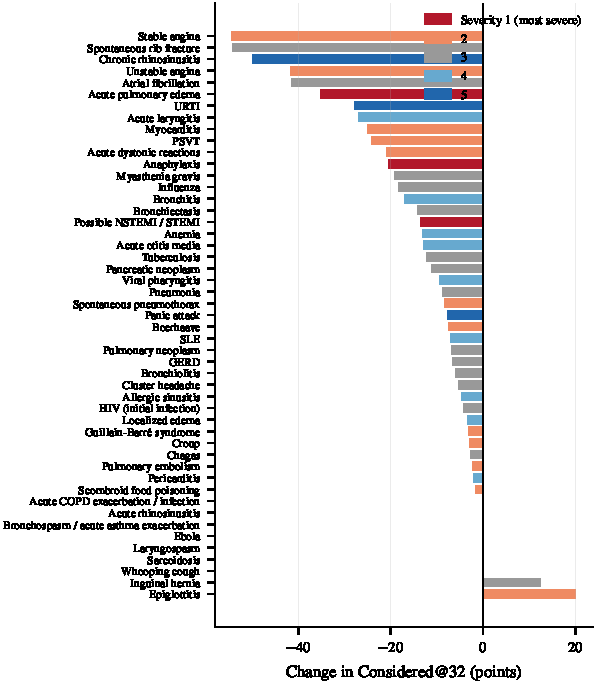
\includegraphics[width=0.55\linewidth]{figures/fig_percond.pdf}
\caption{Change in Considered@32 per condition, Qwen2.5-7B-Instruct minus its base model ($T{=}1$, 980 cases), colored by DDXPlus severity (dark red = most severe). Conditions with fewer than five cases giving them reference probability $\geq 0.1$ are omitted. Angina, acute pulmonary edema, anaphylaxis and myocarditis are among the largest drops.}
\label{fig:percond}
\end{figure}

\subsection{Robustness to prompt and output format}\label{sec:robust}
\paragraph{Prompt.} We repeat the Qwen3-8B pair with two other prompts (Table~\ref{tab:prompts}). \emph{Plain} drops the system prompt and rewords the instructions. \emph{CoT} asks the model to reason step by step before answering; Qwen3's thinking mode stays off in all runs.
The plain prompt reproduces the pattern: the post-trained model gains $+23.0$ $[+20.9,+25.1]$ points at $k{=}1$ and loses $-7.1$ $[-9.3,-5.0]$ at $k{=}32$ ($T{=}0.7$; at $T{=}1$, $+34.2$ and $-8.7$ $[-11.0,-6.4]$), with 1.3--1.5 distinct answers against 3.7--5.6.
Asking for reasoning changes the picture. With CoT, the post-trained model's $\passk{32}$ rises from 0.607 to 0.835: it leads the base model at every $k$ at $T{=}0.7$ ($+4.7$ $[+2.9,+6.6]$ at $k{=}32$) and ties it at $T{=}1$ ($0.0$ $[-2.1,+1.9]$).
Its samples remain far less diverse than the base model's (2.1--2.2 vs.\ 3.9--6.3 distinct answers), so reasoning recovers coverage at $k{=}32$ without restoring sampling diversity.
The coverage loss is therefore largest when the model answers directly, as in most clinical decision-support deployments, and reasoning at inference time mitigates it. This matches the medical models: the reasoning-trained descendants widen the differential (\S\ref{sec:medical}).

\paragraph{Output format.} Base models more often give invalid answers: unparsable, or with a top answer outside the 49 conditions. This affects 12\% of Qwen3-8B-Base samples at $T{=}0.7$ and 25\% at $T{=}1$ (Qwen2.5-7B: 1\% and 21\%), against at most 0.3\% for the post-trained models.
Invalid samples count as wrong, which deflates the base model at large $k$ but inflates the post-trained model's gain at small $k$.
Among valid samples only, the post-trained models still gain $+12.0$ $[+9.8,+14.1]$ (Qwen3, $T{=}0.7$), $+18.7$ $[+16.6,+20.7]$ (Qwen3, $T{=}1$), $+12.2$ $[+10.4,+14.0]$ and $+16.8$ $[+15.0,+18.5]$ points (Qwen2.5) at $k{=}1$, so a quarter to a third of the raw gain at $T{=}1$ is format.
On the cases where every sample of both models is valid, the large-$k$ loss persists: $-15.2$ $[-21.9,-8.6]$ at $k{=}32$ for Qwen3 (105 cases) and $-10.2$ $[-12.7,-7.6]$ for Qwen2.5 (748 cases), both at $T{=}0.7$. (At $T{=}1$ almost no case has 32 valid base samples.) The reported large-$k$ losses are thus lower bounds.

\begin{table}[t]
\centering\small
\begin{adjustbox}{max width=\linewidth}
\begin{tabular}{llcccccc}
\toprule
 & & \multicolumn{2}{c}{pass@1} & \multicolumn{2}{c}{pass@32} & \multicolumn{2}{c}{Distinct} \\
Prompt & $T$ & Base & Post & Base & Post & Base & Post \\
\midrule
default & 0.7 & 0.388 & \textbf{0.558} & \textbf{0.730} & 0.607 & 3.76 & 1.27 \\
default & 1.0 & 0.282 & \textbf{0.556} & \textbf{0.789} & 0.643 & 6.60 & 1.53 \\
plain & 0.7 & 0.352 & \textbf{0.583} & \textbf{0.727} & 0.655 & 3.72 & 1.28 \\
plain & 1.0 & 0.244 & \textbf{0.586} & \textbf{0.792} & 0.705 & 5.57 & 1.54 \\
CoT & 0.7 & 0.409 & \textbf{0.652} & 0.788 & \textbf{0.835} & 3.89 & 2.08 \\
CoT & 1.0 & 0.275 & \textbf{0.642} & 0.837 & 0.837 & 6.31 & 2.24 \\
\bottomrule
\end{tabular}
\end{adjustbox}
\caption{Qwen3-8B-Base vs.\ Qwen3-8B on DDXPlus (980 cases, 32 samples) under three prompts. Bold marks the significantly better model (paired case bootstrap). Without reasoning, the base model wins at $k{=}32$; with CoT, the post-trained model matches or beats it, but its samples stay far less diverse.}
\label{tab:prompts}
\end{table}

\subsection{Which post-training stage narrows the differential?}\label{sec:stages}
The Qwen pairs compare a base model with the end of a post-training pipeline. OLMo~3~\citep{olmo2025olmo3} releases every stage of its 7B instruct pipeline from one base model: supervised fine-tuning, then DPO, then RL with verifiable rewards on math, code, instruction-following and chat prompts (the released OLMo-3-7B-Instruct). It also releases RL-Zero checkpoints trained with RL directly from the base; we use the general one, trained on chat prompts with an LM-judge reward. (The RL-Zero-Mix checkpoint does not load in our vLLM version.) Table~\ref{tab:stages} gives the results.

The coverage loss replicates in this third family. At $T{=}0.7$, every post-trained stage is worse than the base at $k{=}32$: by $-14.6$ $[-17.5,-11.7]$ points after SFT, $-9.2$ $[-12.1,-6.1]$ after DPO, $-28.3$ $[-31.5,-25.0]$ after RLVR, and $-13.3$ $[-16.1,-10.5]$ for RL-Zero. Diversity falls at every stage of the pipeline, from 4.93 distinct answers for the base to 4.01 after SFT, 3.30 after DPO and 2.37 after RLVR.

Compared stage to stage, DPO recovers part of what SFT lost at large $k$ ($+5.4$ $[+2.9,+8.0]$ points at $k{=}32$, and $+10.3$ $[+9.0,+11.6]$ at $k{=}1$) while narrowing the differential further ($-0.71$ distinct answers).
The final RLVR stage is the largest single narrowing. Against the DPO model it loses $-19.1$ $[-21.8,-16.3]$ points at $k{=}32$, 0.92 distinct answers and 7.7 points of coverage@32, and it is also worse at $k{=}1$ ($-5.9$ $[-7.2,-4.6]$). It drops severe-tier Considered@32 to 0.25, a loss of $-16.1$ $[-18.6,-13.5]$ points relative to the base, against $-7.4$ for the DPO model. At $T{=}1$ the pattern is the same (RLVR vs.\ DPO: $-12.7$ $[-15.4,-9.9]$ at $k{=}32$).

RL applied directly to the base narrows the differential less. At $T{=}1$, RL-Zero shows no detectable loss of the base model's $\passk{32}$ ($-1.8$ $[-4.5,+0.8]$, so at most 4.5 points) and 6.28 of its 7.53 distinct answers, and it loses 4.0 $[1.2,6.9]$ points of severe-tier consideration, against 14.4 for the full instruct pipeline. At $T{=}0.7$ it still loses 13.3 points at $k{=}32$, about as much as SFT.

The OLMo base model often breaks the output format: 40\% of its samples are invalid at $T{=}0.7$ and 47\% at $T{=}1$, while unparsable completions are 16--21\% for the SFT model and at most 1.6\% for the later stages. No case has 32 valid base samples, so the all-valid check of \S\ref{sec:robust} is not possible here. Among valid samples, the post-trained models' gains at $k{=}1$ are small ($-1.9$ to $+4.0$ points at $T{=}0.7$, $+1.3$ to $+8.1$ at $T{=}1$), so most of OLMo's raw gain at $k{=}1$ is format. Invalid samples count as misses and are excluded from distinct answers and entropy, so the base model's coverage and diversity are understated and the losses above are conservative.

Across three families, then, the collapse of the sampled differential is not a necessary effect of RL. It accumulates over the instruction-tuning pipeline; in OLMo~3 7B its largest step is RL applied on top of SFT and DPO, but at 32B it is SFT (\S\ref{sec:big32}), so which stage narrows most depends on the recipe. RL applied directly to a base model (OLMo RL-Zero, AlphaMed's base-initialized checkpoint, and our GRPO runs in \S\ref{sec:training}) narrows the differential less.
On Phenopacket Store the instruct pipeline also loses coverage: every stage trails the base model at $k{=}32$ ($-2.0$ $[-3.0,-1.1]$ points after SFT, $-1.5$ after DPO, $-1.4$ after RLVR; all significant), while RL-Zero does not ($-0.6$ $[-1.4,+0.2]$), from a base model at 4.5\% (\S\ref{sec:rare}).

\begin{table}[t]
\centering\small
\begin{adjustbox}{max width=\linewidth}
\begin{tabular}{llcccccc}
\toprule
$T$ & Stage & pass@1 & pass@32 & Distinct & Entropy & Cov@32 & Severe C@32 \\
\midrule
0.7 & Base & 0.178 & \textbf{0.705} & \textbf{4.93} & \textbf{1.16} & \textbf{0.351} & \textbf{0.412} \\
 & SFT & 0.222 & 0.559 & 4.01 & 0.87 & 0.257 & 0.373 \\
 & SFT+DPO & \textbf{0.324} & 0.613 & 3.30 & 0.63 & 0.272 & 0.338 \\
 & SFT+DPO+RLVR (Instruct) & 0.266 & 0.422 & 2.37 & 0.42 & 0.195 & 0.251 \\
 & RL-Zero (RL from base) & 0.295 & 0.572 & 4.06 & 0.84 & 0.286 & 0.326 \\
\midrule
1.0 & Base & 0.128 & \textbf{0.713} & \textbf{7.53} & \textbf{1.66} & \textbf{0.398} & \textbf{0.469} \\
 & SFT & 0.191 & 0.634 & 6.32 & 1.29 & 0.321 & 0.426 \\
 & SFT+DPO & \textbf{0.313} & 0.688 & 4.48 & 0.87 & 0.312 & 0.410 \\
 & SFT+DPO+RLVR (Instruct) & 0.272 & 0.561 & 3.58 & 0.68 & 0.259 & 0.325 \\
 & RL-Zero (RL from base) & 0.279 & 0.695 & 6.28 & 1.21 & 0.367 & 0.429 \\
\bottomrule
\end{tabular}
\end{adjustbox}
\caption{OLMo~3 7B post-training stages on DDXPlus (980 cases, 32 samples). Severe C@32 is severe-tier Considered@32 as in Table~\ref{tab:severity}. Bold marks the best value in each block. Diversity falls at every stage of the instruct pipeline, and the RLVR stage loses the most coverage; RL from the base keeps the base model's pass@32 at $T{=}1$.}
\label{tab:stages}
\end{table}

\subsection{Replication at 32B}\label{sec:big32}
We repeat the DDXPlus comparisons at $T{=}0.7$ with Qwen2.5-32B and its Instruct model, and with every released stage of OLMo~3.1 32B, whose base is OLMo-3-1125-32B; there is no 32B RL-Zero checkpoint (Table~\ref{tab:big32}).
The sampled differential collapses at 32B too, by about half as much. Post-training costs 4.9 $[2.8,7.1]$ points at $\passk{32}$ for Qwen2.5-32B and 4.0 $[2.0,5.9]$ for OLMo~3.1 32B, halves the number of distinct answers (3.78 $\rightarrow$ 1.68 and 4.32 $\rightarrow$ 2.15), and lowers severe-tier consideration by 6.1 and 8.4 points. For Qwen the loss holds on the 421 cases where every base sample is valid ($-4.8$ $[-7.8,-1.7]$); the OLMo 32B base gives invalid answers on 27\% of samples. With few-shot prompts, which nearly remove invalid answers, both losses are three to five times larger (\S\ref{sec:fewshot}).
The stage attribution differs from 7B. In OLMo~3.1 32B the largest narrowing is SFT ($\passk{32}$ $-12.1$ $[-14.4,-9.9]$, distinct answers $-1.39$, severe tier $-11.9$); DPO recovers most of it ($+10.9$ against SFT), and the final RL step is small ($-2.8$ $[-4.3,-1.1]$ at $k{=}32$, $-0.14$ distinct answers). OLMo~3.1 32B and OLMo~3 7B were post-trained with different recipes, so the stage that narrows the samples most is a property of the pipeline, not of SFT, DPO or RL as such.
Under this prompt the stated readout improves in both 32B families (\S\ref{sec:stated}; with few-shot prompts only Qwen2.5-32B's does robustly, \S\ref{sec:fewshot}), and voting stops paying off: majority voting over 32 samples gains the base models 7.0 and 8.4 points and the Instruct models 1.9 and 0.9 (the latter n.s.).

\begin{table}[t]
\centering\small
\setlength{\tabcolsep}{3.5pt}
\begin{adjustbox}{max width=\linewidth}
\begin{tabular}{lcccccccc}
\toprule
Model & pass@1 & pass@32 & Distinct & Cov@32 & Severe C@32 & TV one list$\downarrow$ & TV samples$\downarrow$ & Vote@32 gain \\
\midrule
Qwen2.5-32B (base) & 0.500 & \textbf{0.795} & \textbf{3.78} & \textbf{0.352} & \textbf{0.35} & 0.726 & \textbf{0.726} & $+7.0$ \\
Qwen2.5-32B-Instruct & \textbf{0.604} & 0.746 & 1.68 & 0.276 & 0.29 & \textbf{0.674} & 0.759 & $+1.9$ \\
\midrule
OLMo-3-1125-32B (base) & 0.326 & \textbf{0.796} & \textbf{4.32} & \textbf{0.347} & \textbf{0.39} & 0.746 & \textbf{0.742} & $+8.4$ \\
\quad SFT & 0.461 & 0.674 & 2.94 & 0.265 & 0.27 & 0.736 & 0.776 & $+3.6$ \\
\quad SFT+DPO & \textbf{0.584} & 0.784 & 2.29 & 0.293 & 0.32 & \textbf{0.694} & 0.755 & $+2.1$ \\
\quad SFT+DPO+RLVR (Instruct) & 0.560 & 0.756 & 2.15 & 0.283 & 0.30 & 0.701 & 0.763 & $+0.9$ \\
\bottomrule
\end{tabular}
\end{adjustbox}
\caption{32B replication on DDXPlus ($T{=}0.7$, 980 cases, 32 samples). TV columns: distance to the reference differential of one stated list and of the sampled top-1 answers (\S\ref{sec:stated}). Vote@32 gain: accuracy of the majority answer over 32 samples minus single-call accuracy, in points (\S\ref{sec:consequences}). Bold: best value per family.}
\label{tab:big32}
\end{table}


\section{The stated readout: elicitation, robustness and audit}\label{app:stated}
\subsection{Robustness of the stated readout to elicitation}\label{sec:fullprompt}
The stated readout above uses a five-item list. We repeat the Qwen pairs and OLMo~3 7B's base and Instruct models at $T{=}0.7$ with a prompt that asks for a probability on every one of the 49 conditions, summing to one, and take each sample's top answer to be its highest-probability condition (Table~\ref{tab:fullprompt}).
The results match the short list. After post-training the stated distribution is closer to the reference (TV $-0.052$ for Qwen3-8B, $-0.067$ for Qwen2.5-7B-Instruct, $-0.032$ for OLMo-3-7B-Instruct) while the samples move away ($+0.012$ to $+0.038$).
Qwen3-8B's stated probability again beats agreement over 32 samples ($+0.069$ $[+0.033,+0.104]$), Qwen2.5-7B-Instruct's again does not ($-0.074$), and OLMo-3-7B-Instruct's ties it ($-0.010$; $+0.044$ against five samples). The top three of one full distribution beats the three most frequent of 32 sampled answers for Qwen3-8B ($+14.6$ points) but not for the other two models.

\begin{table}[t]
\centering\small
\setlength{\tabcolsep}{4pt}
\begin{adjustbox}{max width=\linewidth}
\begin{tabular}{lcccccc}
\toprule
 & \multicolumn{2}{c}{TV to reference$\downarrow$} & \multicolumn{3}{c}{AUROC, single-call answer correct} & Top-3: one \\
Model & One distribution & Samples & Stated $p$ & Agree@5 & Agree@32 & dist.\ $-$ 32 samples \\
\midrule
Qwen3-8B-Base & 0.733 & \textbf{0.752} & 0.647 & 0.809 & \textbf{0.845} & $-6.7$ \\
Qwen3-8B & \textbf{0.681} & 0.790 & \textbf{0.717} & 0.609 & 0.647 & $+14.6$ \\
Qwen2.5-7B & 0.769 & \textbf{0.758} & 0.688 & 0.792 & \textbf{0.827} & $-10.2$ \\
Qwen2.5-7B-Instruct & \textbf{0.702} & 0.770 & 0.674 & 0.715 & \textbf{0.748} & $+1.6$ \\
OLMo-3-1025-7B & 0.807 & \textbf{0.766} & 0.610 & 0.744 & \textbf{0.786} & $-15.3$ \\
OLMo-3-7B-Instruct & \textbf{0.775} & 0.787 & 0.749 & 0.705 & \textbf{0.759} & $-9.5$ \\
\bottomrule
\end{tabular}
\end{adjustbox}
\caption{Full-distribution prompt on DDXPlus ($T{=}0.7$, 980 cases): a probability on every condition, top answer = highest stated probability. TV: one sample's stated distribution vs.\ the sampled top-1 answers (bold: better model of each pair). AUROC: bold marks each model's best signal.}
\label{tab:fullprompt}
\end{table}

\subsection{Ruling out format, accuracy and floor effects}\label{sec:statedchecks}
Table~\ref{tab:robust} tests simpler explanations of the stated-list result.
\emph{Format.} The general models' post-trained lists and base-model lists at $T{=}0.7$ are nearly all complete (81--99\% name five on-list conditions with probabilities; Qwen base models at $T{=}1$, 61--62\%; the medical models, 61--80\%). Restricting to complete lists leaves the gaps unchanged (Qwen2.5-7B: 0.779 vs.\ 0.719).
\emph{Accuracy.} A more accurate model puts more stated mass on the true pathology, which the reference also favors. Within samples whose top answer is correct, and within those whose top answer is wrong, the post-trained Qwen list is still closer to the reference ($-0.018$ to $-0.034$ and $-0.036$ to $-0.079$ in TV).
\emph{Floor.} One list can do no better than the reference's own top five, and a finite set of samples no better than as many draws from the reference. Measured as excess over these floors, post-training lowers the list's TV (Qwen3-8B 0.479 $\rightarrow$ 0.435) and raises the samples' (0.557 $\rightarrow$ 0.613).
\emph{True pathology removed.} With the true pathology removed from both list and reference and both renormalized, the post-trained Qwen and OLMo~3.1 32B lists are still closer to the reference ($-0.018$ to $-0.056$), and DDXPlus's set F1 against the reference's support improves by 0.040--0.083 (Table~\ref{tab:clustered}). Since a renormalized list's TV is at least one minus the reference mass it names, TV and mass are not independent evidence; these two controls do not depend on it in the same way.
\emph{Patient-blind list.} A fixed list of the five conditions with the highest average reference probability scores TV 0.794, mass 0.238 and DDF1 0.272; every model's list beats it except OLMo~3 7B's.
\emph{Over-naming.} As a share of named conditions, post-trained lists name fewer that the reference gives less than 1\% (Qwen3-8B 0.59 $\rightarrow$ 0.55) and fewer unwarranted severe conditions (Qwen2.5-32B 0.74 $\rightarrow$ 0.65), but as a count per list the change is mixed: from 0.22 fewer unwarranted severe conditions (OLMo~3.1 32B) to 0.35 more (OLMo~3 7B).
\emph{Severe conditions one by one.} Counting a severe condition wherever the reference gives it any weight, 4--8 of the 17 are named less often after post-training in each pair. Acute pulmonary edema loses most often (Qwen3-8B 0.75 $\rightarrow$ 0.61, Qwen2.5-32B 0.63 $\rightarrow$ 0.44, OLMo~3 7B 0.56 $\rightarrow$ 0.31, OLMo~3.1 32B 0.57 $\rightarrow$ 0.41), followed by stable and unstable angina (Qwen2.5-7B 0.25 $\rightarrow$ 0.08 and 0.19 $\rightarrow$ 0.11), NSTEMI/STEMI (OLMo~3 7B 0.31 $\rightarrow$ 0.14, OLMo~3.1 32B 0.49 $\rightarrow$ 0.36), myocarditis (Qwen2.5-32B 0.14 $\rightarrow$ 0.05) and pulmonary embolism (OLMo~3.1 32B 0.39 $\rightarrow$ 0.31).
\emph{Sampling from the list.} Replacing each sample's top answer with a draw from its own stated list raises $\passk{32}$ for every model. Compared like for like, post-trained lists reach higher than their base model's lists in five of seven comparisons (Qwen3-8B 0.811 vs.\ 0.780 at $T{=}0.7$, Qwen2.5-32B-Instruct 0.880 vs.\ 0.850, OLMo~3.1 32B Instruct 0.853 vs.\ 0.839), but not for Qwen3-8B at $T{=}1$ (0.820 vs.\ 0.832) or OLMo~3 7B (0.577 vs.\ 0.719), and a uniform guesser reaches 0.48.
OLMo~3 7B remains the exception throughout: its Instruct list is closer to the reference when its top answer is correct but much farther when it is wrong.

\begin{table}[t]
\centering\small
\begin{adjustbox}{max width=\linewidth}
\begin{tabular}{lcccccccc}
\toprule
 & Complete & \multicolumn{3}{c}{TV of one list$\downarrow$} & \multicolumn{2}{c}{Excess TV over floor$\downarrow$} & Severe named & pass@32 \\
Model ($T{=}0.7$) & lists & complete only & top-1 right & top-1 wrong & One list & Samples & ref.\ $<0.1$ & list-sampled \\
\midrule
Qwen3-8B-Base & 0.90 & 0.743 & 0.663 & 0.806 & 0.479 & \textbf{0.557} & 0.752 & 0.780 \\
Qwen3-8B & 0.99 & \textbf{0.701} & \textbf{0.646} & \textbf{0.769} & \textbf{0.435} & 0.613 & \textbf{0.680} & \textbf{0.811} \\
Qwen2.5-7B & 0.95 & 0.779 & 0.689 & 0.828 & 0.514 & \textbf{0.575} & 0.823 & 0.772 \\
Qwen2.5-7B-Instruct & 0.91 & \textbf{0.719} & \textbf{0.655} & \textbf{0.773} & \textbf{0.452} & 0.605 & \textbf{0.796} & \textbf{0.802} \\
Qwen2.5-32B & 0.96 & 0.725 & 0.661 & 0.795 & 0.462 & \textbf{0.543} & 0.735 & 0.850 \\
Qwen2.5-32B-Instruct & 0.98 & \textbf{0.674} & \textbf{0.639} & \textbf{0.726} & \textbf{0.409} & 0.579 & \textbf{0.645} & \textbf{0.880} \\
\midrule
OLMo-3-1025-7B & 0.81 & \textbf{0.794} & 0.687 & \textbf{0.837} & \textbf{0.524} & \textbf{0.522} & \textbf{0.747} & \textbf{0.719} \\
OLMo-3-7B-Instruct & 0.95 & 0.823 & \textbf{0.659} & 0.882 & 0.558 & 0.671 & 0.779 & 0.577 \\
OLMo-3-1125-32B & 0.89 & 0.744 & 0.662 & 0.812 & 0.481 & \textbf{0.532} & 0.706 & 0.839 \\
OLMo-3.1-32B-Instruct & 0.99 & \textbf{0.701} & \textbf{0.644} & \textbf{0.774} & \textbf{0.436} & 0.583 & \textbf{0.634} & \textbf{0.853} \\
\bottomrule
\end{tabular}
\end{adjustbox}
\caption{Robustness of the stated-list result (DDXPlus, $T{=}0.7$, 980 cases, valid samples). Complete lists: share naming five on-list conditions with valid probabilities. TV of one list on complete lists only, and on samples whose top answer is right or wrong. Excess TV: TV minus the expected TV of the matching oracle (the reference's top five for one list; as many reference draws as the model has valid samples for the samples). Severe named, ref.\ $<0.1$: share of named severe conditions that the reference gives less than 0.1 (over-naming). pass@32 list-sampled: top answers drawn from each sample's stated list. Bold: better model of each pair. Excess TV is averaged over samples against each case's floor, so it is not exactly the difference of the mean TV and the mean floor. A uniform guesser scores about 0.48 at pass@32.}
\label{tab:robust}
\end{table}

\subsection{Few-shot elicitation}\label{sec:fewshot}
The main analyses give every model the same zero-shot chat prompt, which base models were not trained to follow; they give invalid answers on up to 47\% of samples, which we count as wrong. We therefore re-ran the five final base/post-trained pairs at $T{=}0.7$ with three worked examples in the prompt: three fixed DDXPlus training patients with different true pathologies, each followed by the top five conditions of its reference differential, with probabilities, in the JSON format the instructions ask for. Base models see the instructions and examples as a plain document and complete the next one (generation stops at the end of the list); post-trained models see the same instructions and examples as earlier chat turns. Invalid samples fall below 0.5\% for every model (Table~\ref{tab:fewshot}).

The examples help base models most. Their pass@1 rises from 0.178 to 0.306 for OLMo-3-1025-7B, from 0.326 to 0.528 for OLMo-3-1125-32B and from 0.500 to 0.647 for Qwen2.5-32B, and their pass@32 reaches 0.76--0.90, while their stated lists barely change (TV 0.712--0.787, against 0.726--0.794 zero-shot). The losses in the samples therefore grow (Table~\ref{tab:fewshotdiff}): post-training costs 15.2--29.9 points of pass@32 in every pair, including both 32B pairs, whose zero-shot losses did not survive correction, and every post-trained model's Cov@32 (0.21--0.25) is below every base model's (0.33--0.45) and below a uniform guesser's.

For the three Qwen pairs the stated-list improvement persists and mostly grows: TV $-0.057$ to $-0.087$, $-0.055$ to $-0.073$ with the true pathology removed, and DDF1 $+0.051$ to $+0.081$, all surviving correction. OLMo~3 7B remains the exception (TV $+0.021$, n.s.; $+0.024$ without the true pathology). For OLMo~3.1 32B the improvement shrinks: the post-trained list still places more reference mass on the conditions it names ($+0.047$), but its TV ($-0.022$), TV without the true pathology ($-0.006$) and DDF1 ($+0.009$) no longer survive correction. At 32B the stated-list result is therefore robust for Qwen2.5-32B but depends on the prompt for OLMo~3.1 32B. Post-trained lists still name 5--10 of the 17 severe conditions less often than their base model's.

The consequences replicate in all five pairs. Majority voting over 32 samples gains base models 6.2--10.9 points and post-trained models 0.2--1.1. The three most frequent of 32 sampled answers beat the top three of one stated list by 8.2--22.0 points for base models, while for post-trained models the list is ahead by 0.2--16.7. Agreement with four more samples is the better error signal for every base model (AUROC 0.79--0.84, against 0.67--0.73 for the stated probability), and the stated probability for every post-trained model (0.69--0.77, against 0.56--0.68).
This check uses one temperature and one set of examples, and the examples show the reference's own lists, which may help every model match the reference.

\begin{table}[t]
\centering
\begin{adjustbox}{max width=\textwidth}
\begin{tabular}{lrrrrrrrrrrrr}
\toprule
 & Invalid & & & & \multicolumn{2}{c}{TV, one list} & & TV & Vote@32 & Top-3 list & \multicolumn{2}{c}{AUROC} \\
Model & (\%) & pass@1 & pass@32 & Cov@32 & all & w/o true & DDF1 & samples & gain & $-$ samples & stated & agree@5 \\
\midrule
Qwen3-8B-Base & 0.1 & 0.403 & \textbf{0.809} & \textbf{0.383} & 0.768 & 0.860 & 0.245 & \textbf{0.732} & $+8.4$ & $-16.0$ & 0.722 & 0.828 \\
Qwen3-8B & 0.0 & \textbf{0.601} & 0.639 & 0.221 & \textbf{0.682} & \textbf{0.805} & \textbf{0.327} & 0.786 & $+0.2$ & $+14.5$ & 0.693 & 0.563 \\
\midrule
Qwen2.5-7B (base) & 0.4 & 0.398 & \textbf{0.761} & \textbf{0.333} & 0.784 & 0.879 & 0.238 & \textbf{0.756} & $+6.2$ & $-15.6$ & 0.734 & 0.792 \\
Qwen2.5-7B-Instruct & 0.0 & \textbf{0.450} & 0.535 & 0.220 & \textbf{0.702} & \textbf{0.806} & \textbf{0.309} & 0.798 & $+0.6$ & $+16.7$ & 0.757 & 0.594 \\
\midrule
Qwen2.5-32B (base) & 0.1 & 0.647 & \textbf{0.896} & \textbf{0.343} & 0.712 & 0.847 & 0.298 & \textbf{0.715} & $+7.1$ & $-8.2$ & 0.726 & 0.838 \\
Qwen2.5-32B-Instruct & 0.0 & \textbf{0.663} & 0.744 & 0.252 & \textbf{0.654} & \textbf{0.775} & \textbf{0.349} & 0.758 & $+0.6$ & $+10.1$ & 0.718 & 0.647 \\
\midrule
OLMo-3-1025-7B (base) & 0.2 & 0.306 & \textbf{0.857} & \textbf{0.454} & \textbf{0.787} & \textbf{0.859} & \textbf{0.245} & \textbf{0.712} & $+10.9$ & $-22.0$ & 0.674 & 0.823 \\
OLMo-3-7B-Instruct & 0.1 & \textbf{0.338} & 0.558 & 0.213 & 0.808 & 0.884 & 0.238 & 0.830 & $+0.7$ & $+0.2$ & 0.733 & 0.668 \\
\midrule
OLMo-3-1125-32B (base) & 0.4 & 0.528 & \textbf{0.888} & \textbf{0.397} & 0.719 & 0.818 & 0.302 & \textbf{0.699} & $+8.9$ & $-13.4$ & 0.670 & 0.826 \\
OLMo-3.1-32B-Instruct & 0.0 & \textbf{0.575} & 0.697 & 0.249 & \textbf{0.697} & \textbf{0.812} & \textbf{0.311} & 0.772 & $+1.1$ & $+3.7$ & 0.772 & 0.684 \\
\bottomrule
\end{tabular}
\end{adjustbox}
\caption{Few-shot elicitation on DDXPlus ($T{=}0.7$, 980 cases, 32 samples; three worked examples in the prompt for every model, \S\ref{sec:fewshot}). Invalid: samples naming no listed condition. TV: distance to the reference differential, for one stated list (with the true pathology removed from both in ``w/o true'') and for the sampled top answers. Vote@32 gain and top-3 list minus top-3 of the samples are in accuracy points. AUROC: for the single-call answer being correct, of its stated probability and of agreement with the next 4 samples. Bold: better of the pair.}
\label{tab:fewshot}
\end{table}

\begin{table}[t]
\centering
\begin{adjustbox}{max width=\textwidth}
\begin{tabular}{lllllll}
\toprule
 & pass@32 & TV & \multicolumn{2}{c}{TV, one list} & & Reference mass \\
Pair (base $\rightarrow$ post) & (points) & samples & all & w/o true & DDF1 & of one list \\
\midrule
Qwen3-8B & $-12.4$ / $-17.0$ & $+0.043$ / $+0.054$ & $-0.043$ / $-0.087$ & $-0.018$$^{\dagger}$ / $-0.055$ & $+0.042$ / $+0.081$ & $+0.062$ / $+0.113$ \\
Qwen2.5-7B & $-9.7$ / $-22.7$ & $+0.028$$^{\dagger}$ / $+0.042$ & $-0.062$ / $-0.082$ & $-0.041$ / $-0.073$ & $+0.062$ / $+0.072$ & $+0.073$ / $+0.124$ \\
Qwen2.5-32B & $-4.9$$^{\dagger}$ / $-15.2$ & $+0.033$ / $+0.044$ & $-0.053$ / $-0.057$ & $-0.043$ / $-0.072$ & $+0.051$ / $+0.051$ & $+0.067$ / $+0.084$ \\
OLMo~3 7B & $-28.3$ / $-29.9$ & $+0.090$ / $+0.118$ & $+0.029$$^{\dagger}$ / $+0.021$$^{\dagger}$ & $+0.034$ / $+0.024$ & $-0.006$$^{\dagger}$ / $-0.007$$^{\dagger}$ & $-0.010$$^{\dagger}$ / $-0.002$$^{\dagger}$ \\
OLMo~3.1 32B & $-4.0$$^{\dagger}$ / $-19.1$ & $+0.020$$^{\dagger}$ / $+0.074$ & $-0.045$ / $-0.022$$^{\dagger}$ & $-0.023$ / $-0.006$$^{\dagger}$ & $+0.040$ / $+0.009$$^{\dagger}$ & $+0.056$ / $+0.047$ \\
\bottomrule
\end{tabular}
\end{adjustbox}
\caption{Base $\rightarrow$ post-trained differences under the zero-shot prompt / the few-shot prompt (DDXPlus, $T{=}0.7$). $^{\dagger}$: not significant under the condition-clustered bootstrap with Holm correction (over 112 tests for the zero-shot and 70 for the few-shot pairs; Appendix~\ref{app:clustered}).}
\label{tab:fewshotdiff}
\end{table}

\subsection{A third family: Mistral-7B v0.3}\label{sec:mistral}
We repeat the comparison with Mistral-7B-v0.3 and Mistral-7B-Instruct-v0.3, a family also studied by \citet{jang2026cannotsample}. With the zero-shot prompt the base model does not answer: 52\% of its samples at $T{=}0.7$ and 76\% at $T{=}1$ are invalid (it continues the document instead), and its valid answers mostly repeat the first listed condition, so its single-call accuracy is 6\% and the zero-shot pair is not informative. With the few-shot prompt of \S\ref{sec:fewshot} the base model answers validly (0.4\% invalid), and the pair reproduces the other families (Table~\ref{tab:third}). Post-training raises pass@1 by 14.0 points and lowers pass@32 by 14.5, cuts distinct answers from 5.0 to 1.3 and Cov@32 by 0.138, and moves the samples away from the reference (TV $+0.058$). Voting gains the base model 5.6 points and the Instruct model 0.8; the three most frequent of 32 samples beat one list by 12.6 points for the base model, while for the Instruct model the list is ahead by 7.0; agreement is the better error signal for the base model (AUROC 0.826 against 0.671) and the stated probability for the Instruct model (0.747 against 0.613). The stated list improves modestly (TV $-0.036$, $-0.023$ with the true pathology removed, DDF1 $+0.046$, all surviving clustering and Holm correction over 70 tests), the smallest gain of the three families, and 11 of the 17 severe conditions are named less often. Mistral-Instruct also names 0.4 conditions per list that are not among the 49.

\subsection{Thinking mode}\label{sec:thinking}
Qwen3-8B can reason in a thinking block before it answers; the main runs turn this off. With thinking on (zero-shot prompt, $T{=}0.7$, up to 8,192 tokens; traces average about 1,500 tokens and all end before the limit), the same weights behave differently (Table~\ref{tab:third}). Accuracy rises at both ends: pass@1 is 0.671 against 0.559 without thinking, and pass@32 is 0.815, above both the non-thinking model (0.607) and the base model (0.732; $+8.4$ points, surviving correction). The samples are still narrow (1.76 distinct answers against 3.77 for the base model; Cov@32 0.283 against 0.323) but no farther from the reference than the base model's (TV 0.745 against 0.750). The stated list is the closest of any 7--8B model (TV 0.670, against 0.700 without thinking). The shift in error signals reverses: agreement is again the better signal (AUROC 0.693 with five samples, against 0.638 for the stated probability), as for base models, and voting gains 1.5 points (n.s.). The narrowing of the samples and the advantage of the stated probability are therefore properties of answering directly, which a reasoning mode largely undoes, consistent with the chain-of-thought prompt of \S\ref{sec:robust}.

\subsection{Averaging stated lists across calls}\label{sec:aggregate}
Stated lists can be averaged across calls, as samples can be voted. For each case we average the first 5 or 32 valid stated lists, each renormalized over the conditions it names, and score the mean against the reference (Table~\ref{tab:aggregate}). Averaging helps base models far more than post-trained ones, whose lists vary little between calls (with the zero-shot prompt, 32 averaged lists name 7.6--13.4 conditions, against 16.6--28.8 for base models). The mean of five base-model lists is about as close to the reference as one post-trained list (Qwen3-8B 0.699 against 0.701, Qwen2.5-7B 0.717 against 0.716, OLMo~3.1 32B 0.691 against 0.701). With five lists on both sides, the post-trained mean is closer for Qwen2.5-7B under both prompts ($-0.025$ and $-0.027$) and for Qwen2.5-32B and Qwen3-8B under one prompt each, not significantly closer for OLMo~3.1 32B (zero-shot) and Mistral (few-shot), and farther for OLMo~3 7B and few-shot OLMo~3.1 32B. Averaged base lists also name severe conditions at least as often, and more often for OLMo~3.1 32B, OLMo~3 7B, Mistral and few-shot Qwen2.5-32B (by 0.06--0.14). Direct-answer post-training thus mostly packs into one call the differential that the base model spreads across calls, as \citet{lake2025overton} find for opinions, rather than adding information that averaged base lists lack. Qwen3-8B's thinking mode is the exception: five of its lists beat five base-model lists (TV $-0.049$) and name more severe conditions ($+0.129$). For a post-trained model answering directly, averaging five lists instead of reading one improves TV by only 0.006--0.040; it names 6--17 points more severe conditions, mostly by naming one to three more conditions. Five post-trained lists still cover 0.44--0.50 of the reference mass at $T{=}0.7$ (OLMo~3 7B 0.37) with six to eight conditions, about twice what their 32 samples cover (0.22--0.28) and as much as a uniform guesser naming about 24 conditions (0.48), so the coverage deficit of \S\ref{sec:sampled} is one of the sampled readout.

\begin{table}[t]
\centering
\begin{adjustbox}{max width=\textwidth}
\begin{tabular}{lrrrrrrrrrrrrr}
\toprule
 & Invalid & & & & & \multicolumn{2}{c}{TV, one list} & & TV & Vote@32 & Top-3 list & \multicolumn{2}{c}{AUROC} \\
Model & (\%) & pass@1 & pass@32 & Distinct & Cov@32 & all & w/o true & DDF1 & samples & gain & $-$ samples & stated & agree@5 \\
\midrule
Mistral-7B-v0.3 (base), few-shot & 0.4 & 0.428 & \textbf{0.791} & \textbf{5.02} & \textbf{0.355} & 0.777 & 0.875 & 0.250 & \textbf{0.741} & $+5.6$ & $-12.6$ & 0.671 & 0.826 \\
Mistral-7B-Instruct-v0.3, few-shot & 0.3 & \textbf{0.568} & 0.646 & 1.34 & 0.217 & \textbf{0.741} & \textbf{0.851} & \textbf{0.296} & 0.799 & $+0.8$ & $+7.0$ & 0.747 & 0.613 \\
\midrule
Qwen3-8B-Base & 11.3 & 0.388 & 0.732 & \textbf{3.77} & \textbf{0.323} & 0.743 & 0.833 & 0.276 & 0.750 & $+3.4$ & $-7.3$ & 0.595 & 0.772 \\
Qwen3-8B, non-thinking & 0.0 & 0.559 & 0.607 & 1.27 & 0.217 & 0.700 & 0.815 & 0.318 & 0.793 & $+0.3$ & $+13.7$ & 0.734 & 0.613 \\
Qwen3-8B, thinking & 0.0 & \textbf{0.671} & \textbf{0.815} & 1.76 & 0.283 & \textbf{0.670} & \textbf{0.799} & \textbf{0.349} & \textbf{0.745} & $+1.5$ & $+3.0$ & 0.638 & 0.693 \\
\bottomrule
\end{tabular}
\end{adjustbox}
\caption{A third family and a reasoning mode on DDXPlus ($T{=}0.7$, 980 cases, 32 samples). Top: Mistral-7B v0.3 with the few-shot prompt of \S\ref{sec:fewshot}. Bottom: Qwen3-8B-Base and Qwen3-8B with thinking off (the main runs) and on, with the zero-shot prompt. Columns as in Table~\ref{tab:fewshot}; Distinct: distinct top answers per 32 samples. Bold: best within each block.}
\label{tab:third}
\end{table}

\begin{table}[t]
\centering
\begin{adjustbox}{max width=\textwidth}
\begin{tabular}{lrrrrrrrr}
\toprule
 & \multicolumn{3}{c}{TV, base model} & \multicolumn{3}{c}{TV, post-trained model} & \multicolumn{2}{c}{Post $-$ base, 5 lists each} \\
Pair & 1 list & mean of 5 & mean of 32 & 1 list & mean of 5 & mean of 32 & TV & Severe named \\
\midrule
\multicolumn{9}{l}{\emph{Zero-shot prompt}} \\
Qwen3-8B & 0.732 & 0.699 & 0.691 & 0.701 & 0.695 & 0.692 & $-0.004$$^{\dagger}$ & $+0.030$$^{\dagger}$ \\
Qwen2.5-7B & 0.773 & 0.717 & 0.706 & 0.716 & 0.692 & 0.685 & $-0.025$ & $+0.023$$^{\dagger}$ \\
Qwen2.5-32B & 0.728 & 0.681 & 0.674 & 0.674 & 0.658 & 0.654 & $-0.024$ & $-0.037$$^{\dagger}$ \\
OLMo~3 7B & 0.796 & 0.730 & 0.717 & 0.823 & 0.805 & 0.801 & $+0.074$ & $-0.076$ \\
OLMo~3.1 32B & 0.749 & 0.691 & 0.678 & 0.701 & 0.677 & 0.673 & $-0.014$$^{\dagger}$ & $-0.088$ \\
\midrule
\multicolumn{9}{l}{\emph{Few-shot prompt}} \\
Qwen3-8B & 0.767 & 0.704 & 0.689 & 0.680 & 0.673 & 0.672 & $-0.030$ & $-0.006$$^{\dagger}$ \\
Qwen2.5-7B & 0.782 & 0.712 & 0.694 & 0.703 & 0.686 & 0.683 & $-0.027$ & $+0.012$$^{\dagger}$ \\
Qwen2.5-32B & 0.712 & 0.655 & 0.641 & 0.655 & 0.640 & 0.638 & $-0.015$$^{\dagger}$ & $-0.094$ \\
OLMo~3 7B & 0.787 & 0.703 & 0.676 & 0.806 & 0.786 & 0.778 & $+0.083$ & $-0.141$ \\
OLMo~3.1 32B & 0.719 & 0.651 & 0.630 & 0.697 & 0.682 & 0.680 & $+0.031$ & $-0.060$ \\
Mistral-7B v0.3 & 0.774 & 0.708 & 0.691 & 0.742 & 0.723 & 0.720 & $+0.015$$^{\dagger}$ & $-0.118$ \\
\midrule
\multicolumn{9}{l}{\emph{Zero-shot prompt, thinking on}} \\
Qwen3-8B, thinking & 0.732 & 0.699 & 0.691 & 0.672 & 0.650 & 0.647 & $-0.049$ & $+0.129$ \\
\bottomrule
\end{tabular}
\end{adjustbox}
\caption{Averaging stated lists across calls (DDXPlus, $T{=}0.7$, 980 cases). TV to the reference differential of the first valid stated list (so values differ slightly from averages over all lists elsewhere) and of the mean of the first 5 or 32 valid lists, for the base and the final post-trained model. Last two columns: post-trained minus base with five averaged lists each, for TV and for the share of severe conditions with reference probability $\geq 0.1$ that are named. $^{\dagger}$: the condition-clustered 95\% interval includes zero.}
\label{tab:aggregate}
\end{table}

\subsection{Which signal to use: combination and held-out audit}\label{sec:audit}
Whether the stated probability or agreement across samples is the better error signal varies across models, so we ask what predicts it and whether a practitioner can tell. We pool 56 model--setting combinations scored on DDXPlus: the base/post-trained pairs at both temperatures and with three prompts, the OLMo stages, the 32B models, the medical models, our GRPO runs, and the full-distribution prompt. They share weights, prompts and temperatures, so we treat the correlations below as descriptive.
The stated probability's advantage over five-sample agreement correlates with the \emph{single-answer rate}, the share of cases whose five samples all give the same top answer (Spearman 0.75), with the stated probability's own AUROC (0.82; the gap contains this term, so part of this is by construction), and negatively with the number of distinct answers ($-0.74$). The stated probability is the better signal for 19 of the 56. No single-answer threshold separates them: Qwen2.5-7B-Instruct still favors agreement, while OLMo~3 7B's DPO and Instruct models favor their unusually informative stated probability.
Combining the signals beats choosing between them. Fitting a logistic model of correctness on the stated probability and five-sample agreement with 100 labeled cases, and evaluating on the other 880, gives a mean held-out AUROC of 0.753 for the 39 post-trained combinations (0.765 for all 56); averaging the two signals' ranks without fitting gives 0.746; picking the better single signal on the same 100 cases gives 0.720; always using agreement 0.695; always using the stated probability 0.671. The logistic combination beats the single-signal pick for 35 of the 39 post-trained combinations. This matches the general finding that hybrids of consistency and verbalized confidence beat either~\citep{xiong2024express}.
For choosing a single signal, the simplest rule, always using agreement, is right for 66\% of the combinations (54\% of the 39 post-trained ones) and loses 0.025 AUROC on average (0.032). An audit does better: choose the signal with the higher AUROC on 100 random labeled cases, using five samples per case, and evaluate the choice on the other 880. Over 500 draws per combination it picks the better held-out signal 86\% of the time (82\% for post-trained models) and loses 0.005 AUROC (0.007); with 50 cases, 82\% and 0.010; with 200, 90\% and 0.003. It is reliable when the two signals differ by more than 0.05 AUROC (96\% of draws, 39 combinations) and close to a coin flip when they differ by less than 0.02 (53\%, 5 combinations), where the choice matters least. The audit's main cost is gold labels for 100 cases from the target population, and we validate it only within DDXPlus.


\section{Medical post-training and rare disease}\label{app:medrare}
\subsection{Medical post-training}\label{sec:medical}
Applied after instruction tuning, medical RL does not cost coverage. AlphaMed improves on its parent at every $k$ (Figure~\ref{fig:alphamed}): +3.9 points at $k{=}1$ ($[+2.2,+5.5]$), widening to +8.4 at $k{=}32$ ($[+6.0,+10.6]$). It reaches at least one correct sample for 47 of 49 conditions, against 39 for its parent.
It does not restore breadth, though: distinct answers (1.87 vs.\ 1.82), entropy (0.29 vs.\ 0.30), and coverage (0.27 vs.\ 0.24) stay at the instruction-tuned level, far below the base model.
AlphaMed also names off-list conditions more often than its parent, a mild loss of instruction following.
By condition, AlphaMed slightly \emph{raises} consideration in every severity tier (+2.2 to +4.3 points; Table~\ref{tab:severity}). It still loses acute pulmonary edema (0.31 to 0.13), and it introduces an attractor of its own: spontaneous pneumothorax as the top answer in 10.3\% of samples, against 4.3\% for its parent and a reference rate of 1.0\%.
Medical post-training thus operates on an already collapsed distribution; the collapse comes from the general post-training stage.
The other two descendants go further (Table~\ref{tab:medical}). HuatuoGPT-o1 (SFT then PPO) and m1 (SFT distillation from a reasoning teacher) both \emph{widen} the differential relative to their parent: 2.49 and 3.29 distinct answers vs.\ 1.82, and coverage@32 of 0.31 and 0.33 vs.\ 0.24. Their pass@32 rises by 13.7 $[+11.3,+16.0]$ and 18.1 $[+15.5,+20.7]$ points. m1 gains almost nothing at $k{=}1$ (+0.9, interval includes zero), so its improvement lies entirely in breadth. Both reasoning-trained models are also less calibrated (ECE 0.17 and 0.21 vs.\ 0.11). Medical post-training on an instruction-tuned model thus never adds to the collapse, and reasoning distillation partially reverses it.

\paragraph{Medical RL from the base model.}
Alongside the instruct-initialized AlphaMed-7B, the AlphaMed authors released a companion checkpoint, AlphaMed-7B-base-rl, initialized from Qwen2.5-7B rather than Qwen2.5-7B-Instruct (according to its configuration file). The paper~\citep{liu2025alphamed} describes only the instruct-initialized models: GRPO with a binary correctness reward on about 19k multiple-choice questions from MedQA and MedMCQA, with a 64-question by 8-sample batch for 300 steps. It does not document the base-initialized checkpoint, so we cannot rule out differences in data or hyperparameters, and we treat it as corroborating rather than controlled evidence.
It offers a third-party check on whether RL itself causes the collapse (Table~\ref{tab:medical}, lower block).
It does not. RL from the base model improves on the base at every $k$ ($+14.3$ $[+13.1,+15.7]$ points at $k{=}1$, $+9.5$ $[+7.4,+11.6]$ at $k{=}32$). It keeps 3.14 distinct answers, against 1.87 for the instruct-initialized AlphaMed.
Against that instruct-model AlphaMed, it is 2.2 $[0.4,3.9]$ points worse at $k{=}1$ and 10.8 $[+8.6,+13.2]$ points better at $k{=}32$.
Its severe-tier Considered@32 shows no detectable change relative to the base ($-0.7$ $[-3.0,+1.7]$ points), against $-12.4$ for instruction tuning and $-8.1$ for instruction tuning followed by AlphaMed's RL (Table~\ref{tab:severity}; all well below the chance levels of \S\ref{sec:collapse}).
This is consistent with our own controlled GRPO-from-base result (\S\ref{sec:training}): with a verifiable correctness reward, RL from a base model buys accuracy without the collapse, which is introduced by general instruction tuning and inherited by everything trained on top of it. OLMo~3 refines this (\S\ref{sec:stages}): within its instruct pipeline, the RL stage applied after SFT and DPO is the largest single narrowing.

\begin{table}[t]
\centering\small
\begin{adjustbox}{max width=\linewidth}
\begin{tabular}{llcccccc}
\toprule
Model & Post-training & pass@1 & pass@32 & Distinct & Entropy & Cov@32 & ECE \\
\midrule
Qwen2.5-7B-Instruct & (parent) & 0.478 & 0.598 & 1.82 & 0.30 & 0.239 & \textbf{0.106} \\
AlphaMed-7B & rule-based RL & 0.516 & 0.682 & 1.87 & 0.28 & 0.266 & 0.121 \\
HuatuoGPT-o1-7B & SFT + PPO & \textbf{0.536} & 0.735 & 2.49 & 0.44 & 0.306 & 0.168 \\
m1-7B-23K & SFT distillation & 0.486 & 0.779 & 3.29 & 0.62 & 0.328 & 0.206 \\
\midrule
Qwen2.5-7B (base) & (parent) & 0.352 & 0.695 & \textbf{4.91} & \textbf{1.00} & \textbf{0.335} & 0.291 \\
AlphaMed-7B (base-RL) & rule-based RL & 0.495 & \textbf{0.790} & 3.14 & 0.62 & 0.320 & 0.202 \\
\bottomrule
\end{tabular}
\end{adjustbox}
\caption{Medical models on DDXPlus (980 cases, 32 samples, $T{=}0.7$). Upper block: descendants of Qwen2.5-7B-Instruct; none narrows the differential further, and the reasoning-trained models widen it. Lower block: AlphaMed's companion checkpoint trained from the base model, which keeps most of the base model's diversity and has the best pass@32 of any 7B model.}
\label{tab:medical}
\end{table}

\begin{figure}[t]
\centering
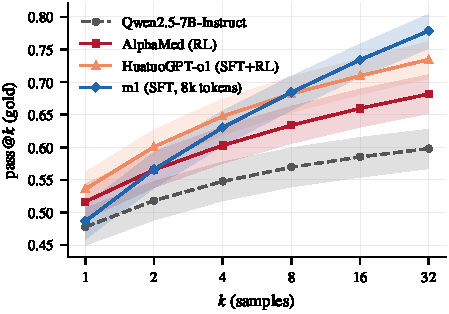
\includegraphics[width=0.5\linewidth]{figures/fig_passk_medical.pdf}
\caption{DDXPlus at $T{=}0.7$ (980 cases): Qwen2.5-7B-Instruct (dashed) vs.\ its medical descendants, with 95\% case-bootstrap bands. Every descendant matches or beats its parent at every $k$, and the gaps widen with $k$: there is no sharpening tax at the medical stage.}
\label{fig:alphamed}
\end{figure}

\subsection{Rare disease: overconfidence without accuracy}\label{sec:rare}
On 1,401 Phenopacket Store cases covering 749 diseases, every 7--8B model is near the floor: $\passk{1}$ is 1.4--2.2\% and $\passk{32}$ is 3.7--7.0\%.
Stated confidence is not near the floor. Qwen2.5-7B-Instruct states a mean top-1 probability of 0.51, and its RL-trained medical descendants state 0.67 (HuatuoGPT-o1) and 0.69 (AlphaMed), while their accuracy is about 2\%. ECE accordingly rises from 0.49 to 0.64--0.67; at this accuracy ECE mostly restates mean confidence, so we read it as a rise in confidence without a matching rise in accuracy.
The RL-trained medical models (AlphaMed; HuatuoGPT-o1 after SFT) thus state much higher confidence where they are least accurate. The effect also appears without instruction tuning: AlphaMed's base-initialized checkpoint is the most overconfident model we evaluate (mean confidence 0.71, ECE 0.70, accuracy 1.7\%).
The medical descendants do gain a little accuracy: AlphaMed beats its parent at every $k$ ($+0.6$ $[+0.2,+0.9]$ points at $k{=}1$, $+1.0$ $[+0.1,+2.1]$ at $k{=}32$), HuatuoGPT-o1 at $k \le 8$, and m1 at $k \ge 2$ ($+1.4$ $[+0.4,+2.5]$ at $k{=}32$). These gains are an order of magnitude smaller than the rise in confidence.
m1, trained only with supervised reasoning traces (at its intended 8k-token budget), is the exception on calibration and diversity: it is the most diverse model (15.3 distinct answers per 32 samples, against 11.5 for the parent and 9.2 for HuatuoGPT-o1), and its confidence rises least (0.57).

General post-training reproduces the DDXPlus pattern on Qwen3. Qwen3-8B beats its base at $\passk{1}$ ($+0.7$ $[+0.4,+1.1]$) and trails it from $k{=}8$ on, by $-2.2$ $[-3.1,-1.3]$ points at $\passk{32}$ (a relative loss of 37\%), with half the distinct answers (6.4 vs.\ 13.4). For Qwen2.5 no pass@$k$ difference is significant.
Unlike medical RL, general post-training \emph{lowers} stated confidence here (0.61 to 0.46 for Qwen3, 0.61 to 0.51 for Qwen2.5), although base models also give invalid answers more often (8.5\% of Qwen3-8B-Base samples).
OLMo~3 does not share this: every stage of its pipeline states a mean confidence of 0.73--0.84 at about 1\% accuracy ($\passk{32}$ 2.5--4.5\%), and its SFT checkpoint is the most overconfident model we evaluate (confidence 0.84, ECE 0.83).
On the 500-case subset, our 8B GRPO runs (\S\ref{sec:training}) are indistinguishable from their base (all pass@$k$ differences within $\pm0.6$ points).

Accuracy depends strongly on when the source case report was published (Table~\ref{tab:era}). For every model, $\passk{32}$ is 5--10\% on cases published up to 2022 ($n{=}901$), at most 1.7\% on 2023--24 cases ($n{=}348$), and 2.6--4.6\% on 2025+ cases ($n{=}152$). The pattern is not monotone, since 2025+ cases score above 2023--24 cases, so case mix also matters; the gap between older and recent cases is consistent with, but does not establish, memorization of older case reports.

\begin{table}[t]
\centering\small
\begin{adjustbox}{max width=\linewidth}
\begin{tabular}{lcccccc}
\toprule
 & \multicolumn{2}{c}{$\le$2022 ($n{=}901$)} & \multicolumn{2}{c}{2023--24 ($n{=}348$)} & \multicolumn{2}{c}{2025+ ($n{=}152$)} \\
Model & pass@1 & pass@32 & pass@1 & pass@32 & pass@1 & pass@32 \\
\midrule
Qwen2.5-7B (base) & 2.0 & 8.2 & 0.0 & 0.3 & 0.6 & 3.3 \\
Qwen2.5-7B-Instruct & 2.3 & 7.7 & 0.0 & 0.9 & 0.8 & 3.9 \\
AlphaMed-7B & 3.0 & 9.0 & 0.3 & 1.4 & 1.4 & 3.9 \\
AlphaMed-7B (base-RL) & 2.4 & 8.8 & 0.1 & 1.1 & 1.4 & 4.6 \\
HuatuoGPT-o1-7B & 3.1 & 8.4 & 0.3 & 1.4 & 1.3 & 3.9 \\
m1-7B & 2.6 & 9.5 & 0.3 & 1.7 & 1.0 & 3.9 \\
Qwen3-8B-Base & 2.1 & 8.3 & 0.1 & 0.6 & 1.1 & 3.9 \\
Qwen3-8B & 3.1 & 5.2 & 0.1 & 0.3 & 2.0 & 2.6 \\
\bottomrule
\end{tabular}
\end{adjustbox}
\caption{Phenopacket Store accuracy (\%, exact diagnosis) by publication year of the source case report (1,401 cases, 32 samples, $T{=}0.7$). Every model is far more accurate on cases published up to 2022 than on 2023--24 cases; 2025+ cases fall in between.}
\label{tab:era}
\end{table}

\subsection{Stated and sampled readouts on real rare-disease cases}\label{sec:phenoreadouts}
Phenopacket Store cases are real, but they have no reference differential and accuracy is near the floor, so we can test only the consequences of \S\ref{sec:consequences}, and we count an answer as correct if it is the diagnosis or a closely related Mondo class (exact matches give only 8--31 correct single-call answers per model). Top answers are grouped by Mondo class for voting and agreement (Table~\ref{tab:pheno}).
The DDXPlus shifts reappear, without a crossover. Majority voting over 32 samples helps the base models by 3.1--4.6 points but the final post-trained models by only 0.4--1.5 (Qwen3-8B $+0.4$, n.s.). Post-training weakens agreement as an error signal (Qwen3-8B 0.830 $\rightarrow$ 0.763, Qwen2.5-7B 0.845 $\rightarrow$ 0.745, OLMo~3 7B 0.814 $\rightarrow$ 0.726) and strengthens the stated probability (0.567 $\rightarrow$ 0.707, 0.598 $\rightarrow$ 0.717, 0.464 $\rightarrow$ 0.652). Agreement beats the stated probability by 0.25--0.35 AUROC for the base models and by only 0.03--0.07 for the post-trained ones, significantly only for Qwen3-8B ($-0.056$ $[-0.120,-0.002]$). On these open-ended cases the three most frequent of 32 sampled answers still contain a correct diagnosis more often than one list's top three, but the gap shrinks from 4.6--7.0 points for the base models to 2.7--3.6 for Qwen2.5-7B-Instruct and OLMo-3-7B-Instruct and to a tie for Qwen3-8B ($+0.4$ $[-0.8,+1.8]$). The medical models behave like their post-trained parent, with agreement the better signal for all of them.

\begin{table}[t]
\centering\small
\begin{adjustbox}{max width=\linewidth}
\begin{tabular}{lccccccc}
\toprule
 & Single-call & Vote@32 & Top-3: list & \multicolumn{3}{c}{AUROC, single-call answer correct} & Correct \\
Model & correct & gain & $-$ 32 samples & Stated $p$ & Agree@5 & Agree@32 & answers \\
\midrule
Qwen3-8B-Base & 0.074 & $+4.6$ & $-7.0$ & 0.567 & 0.768 & \textbf{0.830} & 104 \\
Qwen3-8B & 0.080 & $+0.4$ & $+0.4$ & 0.707 & 0.726 & \textbf{0.763} & 112 \\
Qwen2.5-7B & 0.062 & $+3.8$ & $-5.4$ & 0.598 & 0.788 & \textbf{0.845} & 87 \\
Qwen2.5-7B-Instruct & 0.056 & $+1.5$ & $-3.6$ & 0.717 & 0.661 & \textbf{0.745} & 78 \\
\midrule
OLMo-3-1025-7B & 0.060 & $+3.1$ & $-4.6$ & 0.464 & 0.765 & \textbf{0.814} & 84 \\
\quad SFT & 0.035 & $+1.1$ & $-3.6$ & 0.628 & 0.730 & \textbf{0.814} & 49 \\
\quad SFT+DPO & 0.026 & $+1.2$ & $-3.3$ & 0.651 & 0.673 & \textbf{0.725} & 36 \\
\quad SFT+DPO+RLVR (Instruct) & 0.035 & $+0.9$ & $-2.7$ & 0.652 & 0.644 & \textbf{0.726} & 49 \\
\quad RL-Zero (from base) & 0.065 & $+2.3$ & $-3.1$ & 0.583 & 0.791 & \textbf{0.827} & 91 \\
\midrule
AlphaMed-7B & 0.071 & $+1.6$ & $-3.0$ & 0.586 & 0.755 & \textbf{0.797} & 100 \\
HuatuoGPT-o1-7B & 0.093 & $+2.6$ & $-5.7$ & 0.653 & 0.708 & \textbf{0.756} & 130 \\
m1-7B & 0.084 & $+2.9$ & $-7.9$ & 0.650 & 0.747 & \textbf{0.800} & 117 \\
AlphaMed-7B (base-RL) & 0.054 & $+2.5$ & $-4.2$ & 0.672 & 0.733 & \textbf{0.789} & 75 \\
\bottomrule
\end{tabular}
\end{adjustbox}
\caption{Aggregation and uncertainty on Phenopacket Store (1,401 real rare-disease cases, 32 samples, $T{=}0.7$). An answer counts as correct if it is the diagnosis or a closely related Mondo class. Columns as in Table~\ref{tab:consequences}; Correct answers: number of correct single-call answers, the positives for the AUROCs. Bold: best signal.}
\label{tab:pheno}
\end{table}


\section{Training without collapsing the samples}\label{sec:training}
The stated list survives post-training, but sampled diversity still matters: self-consistency and other sampling-based methods depend on it (\S\ref{sec:consequences}), and so does reinforcement learning itself, since GRPO learns nothing from a group whose samples agree.
Can reinforcement learning raise diagnostic accuracy without collapsing the sampled differential? We fine-tune Qwen3-1.7B with GRPO on DDXPlus training patients (9,800 cases, 200 per condition; disjoint from the test split) and evaluate exactly as in \S\ref{sec:setup}.

\paragraph{Setup.}
We train LoRA adapters ($r{=}32$) with GRPO for 200 steps. Each step uses 16 prompts and 16 sampled completions per prompt, generated with vLLM on the same GPU.
A first sweep with a common aggressive configuration (learning rate $2{\times}10^{-5}$, no KL penalty, 8 samples per prompt, per-group reward standardization) was unstable. In three of seven runs, the policy collapsed to an input-independent answer: one condition for 88--100\% of all patients, with completions shrinking to about 25 tokens.
The starting policy is nearly deterministic (token entropy ${\approx}0.06$), so most GRPO groups have zero reward variance, and noisy updates drive the collapse.
We therefore use learning rate $5{\times}10^{-6}$, KL coefficient 0.04, no reward standardization (as in \citet{puri2026beyondmode}), and 16 samples per prompt. A monitor tracks the number of distinct top-1 answers per case within each batch. All runs in this configuration were stable.

\paragraph{Rewards.}
Every recipe includes a format reward: the answer must parse into a list of distinct conditions with valid probabilities.
\texttt{acc} is standard RLVR: 1 if the top-1 answer is the true pathology.
\texttt{dist} adds two per-sample distributional terms to \texttt{acc}: a Brier score of the stated distribution against the truth, and the overlap of the stated distribution with the reference differential.
Both are computed from a \emph{single} completion. They cannot see that the policy gives the same answer in every sample, which is exactly the collapse of \S\ref{sec:collapse}.
\texttt{gm} adds to \texttt{acc} a \emph{group-level} reward over the GRPO group of $n$ samples for a case. If sample $i$'s top-1 answer is $a$, and $k_a$ samples in the group give $a$,
\begin{equation}
r_i^{\mathrm{gm}} = \operatorname{clip}\!\big(n\,p_{\mathrm{ref}}(a) - (k_a - 1),\ 0,\ 1\big),
\end{equation}
where $p_{\mathrm{ref}}$ is the reference differential. This is sample $i$'s marginal contribution to $n\sum_c \min(q_c, p_{\mathrm{ref}}(c))$, the overlap between the group's empirical answer distribution $q$ and the reference. An answer earns credit while its condition is under-represented relative to its reference mass, and none once it is over-represented.
In contrast to multi-answer rewards that score a set inside one completion~\citep{puri2026beyondmode}, \texttt{gm} acts on the distribution of \emph{sampled} answers, the quantity that collapses.
Because the group reward fires only when a group contains dissenting samples, we also test a boosted variant, \texttt{gm}$^{+}$: \texttt{gm} weight 3 and training temperature 1.2.
As baselines we adapt the multi-answer rewards of \citet{puri2026beyondmode} to our prompt. \textsc{Multi-RLVR} scores the share of listed conditions that belong to the reference differential, treated as a set of acceptable answers; \textsc{Multi-RLCR} adds their set-level Brier term on the per-answer probabilities. Both zero the reward for duplicate or invalid answers, as in the original, and use the same format reward, optimizer and settings as our recipes.

\paragraph{Results.}
Table~\ref{tab:training} reports means over two seeds; intervals bootstrap cases and do not include seed-to-seed variation. All our recipes raise top-1 accuracy by 8--10 points; the multi-answer baselines barely move it (below).
The per-sample recipes (\texttt{acc}, \texttt{dist}) slightly \emph{reduce} diversity relative to the starting model, the sharpening documented in \S\ref{sec:general}.
The group reward removes this. \texttt{gm} matches the starting model's diversity, and \texttt{gm}$^{+}$ exceeds it while also being the most accurate recipe.
Against \texttt{acc}, with paired bootstraps over cases averaged over seeds, \texttt{gm}$^{+}$ improves:
\begin{itemize}
\item pass@1 by $+1.6$ $[+1.0,+2.3]$ and pass@32 by $+1.7$ $[+1.0,+2.6]$ points;
\item distinct answers by $+0.10$ $[+0.07,+0.13]$ and entropy by $+0.034$ $[+0.022,+0.047]$;
\item coverage@32 by $+1.5$ $[+1.0,+2.1]$ points, and TV by $-0.014$ $[-0.019,-0.010]$.
\end{itemize}
Plain \texttt{gm} improves on \texttt{acc} in the same direction with smaller margins (e.g.\ pass@1 $+1.0$ $[+0.6,+1.6]$, entropy $+0.013$ $[+0.005,+0.021]$).
Diversity increases monotonically with group-reward pressure, with no accuracy cost.
The set-membership baselines of \citet{puri2026beyondmode} train stably (their reward rises from 0.27--0.31 to 0.32--0.35) but barely change sampled behavior. pass@1 rises by under 1 point over the untrained model, and diversity is unchanged. Against them, \texttt{gm}$^{+}$ is better on every metric, by $+8.9$ $[+7.4,+10.5]$ points at pass@1, $+0.07$ $[+0.03,+0.11]$ distinct answers and $+3.0$ $[+2.3,+3.8]$ points of coverage@32 (vs.\ \textsc{Multi-RLVR}; \textsc{Multi-RLCR} is similar).
What they do improve is the differential written \emph{inside} one completion: the reference mass covered by a single listed differential rises to 0.317 (\textsc{Multi-RLVR}), against 0.300 for \texttt{acc} and 0.309 for \texttt{gm}$^{+}$.
The two objectives are complementary: a set reward shapes the list a model writes, while the group reward shapes which answer it commits to across samples, which is what collapses under post-training.
The absolute effects are modest because the starting policy is already collapsed: there is little exploration for any reward to act on.
None of the recipes changes rare-disease accuracy or confidence on Phenopacket Store, where a 1.7B model is at the floor; the same holds at 8B (\S\ref{sec:rare}).
\paragraph{Starting from a diverse base model.}
The 1.7B experiment starts from an already collapsed instruct model. We therefore repeat the comparison from Qwen3-8B-Base, the diverse base model of \S\ref{sec:general}, with the same recipe and \texttt{acc} vs.\ \texttt{gm}. We compare against Qwen's own post-trained Qwen3-8B (Table~\ref{tab:training8b}; means of two seeds).
Both RL recipes reach nearly the official model's top-1 accuracy (0.537 and 0.539 vs.\ 0.558; \texttt{gm}: $-1.9$ $[-3.9,+0.1]$ points). They keep more than twice its diversity (2.7--2.9 vs.\ 1.27 distinct answers) and beat it by 15--16 points at pass@32 (\texttt{gm}: $+16.3$ $[+14.0,+18.8]$).
In this setting, then, the collapse produced by general post-training is not required for its top-1 accuracy (our runs train on in-distribution DDXPlus data, so this is an existence result, not a like-for-like comparison of recipes).
Both runs still narrow the base model somewhat, and the group reward narrows it less. At equal pass@1 ($+0.2$, n.s.), \texttt{gm} beats \texttt{acc} on distinct answers $+0.14$ $[+0.11,+0.17]$, entropy $+0.035$ $[+0.029,+0.041]$, coverage@32 $+1.1$ $[+0.8,+1.5]$ points, and pass@32 $+1.2$ $[+0.5,+1.9]$. Each seed reproduces the ordering. The severe tier tells the same story (Table~\ref{tab:severity}): official post-training removes 9.8 points of can't-miss consideration, \texttt{acc} 2.8, and \texttt{gm} 1.5 (not significant). Figure~\ref{fig:grpo8b} shows the pass@$k$ curves.

\begin{figure}[t]
\centering
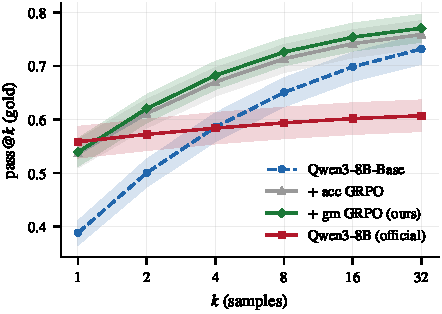
\includegraphics[width=0.5\linewidth]{figures/fig_passk_grpo8b.pdf}
\caption{pass@$k$ on DDXPlus ($T{=}0.7$, 980 cases) from the same pretrained weights: Qwen3-8B-Base, our GRPO runs (pooled over two seeds), and the official post-trained Qwen3-8B, with 95\% case-bootstrap bands. Our RL lifts the whole curve; official post-training trades the right end for the left.}
\label{fig:grpo8b}
\end{figure}

\begin{table}[t]
\centering\small
\begin{adjustbox}{max width=\linewidth}
\begin{tabular}{lcccccc}
\toprule
Model & pass@1 & pass@32 & Distinct & Entropy & Cov@32 & TV$\downarrow$ \\
\midrule
Qwen3-8B-Base (start) & 0.389 & 0.732 & \textbf{3.77} & \textbf{0.78} & \textbf{0.323} & 0.749 \\
\quad + \texttt{acc} GRPO (ours) & 0.537 & 0.759 & 2.72 & 0.52 & 0.297 & 0.750 \\
\quad + \texttt{gm} GRPO (ours) & 0.539 & \textbf{0.770} & 2.86 & 0.56 & 0.308 & \textbf{0.742} \\
Qwen3-8B (official post-training) & \textbf{0.558} & 0.607 & 1.27 & 0.11 & 0.217 & 0.793 \\
\bottomrule
\end{tabular}
\end{adjustbox}
\caption{GRPO from Qwen3-8B-Base vs.\ the official post-trained Qwen3-8B on DDXPlus (980 cases, 32 samples, $T{=}0.7$); GRPO rows are means of two seeds. Our RL nearly matches the official model's top-1 accuracy while keeping more than twice its diversity; the group reward preserves more than \texttt{acc}. The base row comes from this experiment's own sampling run, so it differs slightly from Table~\ref{tab:pairs}.}
\label{tab:training8b}
\end{table}

\begin{table}[t]
\centering\small
\begin{adjustbox}{max width=\linewidth}
\begin{tabular}{lcccccc}
\toprule
Recipe & pass@1 & pass@32 & Distinct & Entropy & Cov@32 & TV$\downarrow$ \\
\midrule
Qwen3-1.7B (untrained) & 0.378 & 0.435 & 1.41 & 0.151 & 0.162 & 0.850 \\
\texttt{acc} & 0.458 & 0.499 & 1.36 & 0.142 & 0.181 & 0.829 \\
\texttt{dist} & 0.458 & 0.502 & 1.34 & 0.131 & 0.181 & 0.829 \\
\textsc{Multi-RLVR}~\citep{puri2026beyondmode} & 0.385 & 0.443 & 1.39 & 0.153 & 0.166 & 0.845 \\
\textsc{Multi-RLCR}~\citep{puri2026beyondmode} & 0.383 & 0.441 & 1.39 & 0.150 & 0.165 & 0.847 \\
\texttt{gm} & 0.469 & 0.510 & 1.40 & 0.155 & 0.186 & 0.825 \\
\texttt{gm}$^{+}$ & \textbf{0.474} & \textbf{0.516} & \textbf{1.46} & \textbf{0.176} & \textbf{0.196} & \textbf{0.815} \\
\bottomrule
\end{tabular}
\end{adjustbox}
\caption{GRPO on Qwen3-1.7B, evaluated on DDXPlus test (980 cases, 32 samples, $T{=}0.7$); means of two seeds. \texttt{gm}$^{+}$: group-reward weight 3, training temperature 1.2. Per-sample rewards slightly narrow the model; set-membership rewards barely move it; the group reward preserves, then widens, its differential while improving accuracy.}
\label{tab:training}
\end{table}

\section{Condition-clustered intervals and multiple comparisons}\label{app:clustered}
DDXPlus has 20 test cases for each of 49 true pathologies, and effects can be specific to a condition, so cases are not independent. Table~\ref{tab:clustered} repeats the headline base-vs-post differences with a bootstrap that resamples the 49 pathologies with all their cases (1,000 resamples), and applies Holm correction across the 112 tests (8 pairs $\times$ 14 metrics). Most differences survive. Those that do not, marked $\dagger$, are the 32B $\passk{32}$ losses, the sampled-TV increases for Qwen2.5-7B and OLMo~3.1 32B, the list changes for OLMo~3 7B, Qwen3-8B's list TV without the true pathology at $T{=}0.7$ (corrected $p{=}0.05$), and the drop in agreement AUROC for both OLMo models.

\begin{table}[t]
\centering\scriptsize
\begin{adjustbox}{max width=\linewidth}
\begin{tabular}{p{2.4cm}p{2.1cm}p{2.1cm}p{2.1cm}p{2.1cm}p{2.1cm}p{2.1cm}p{2.1cm}}
\toprule
Pair (post $-$ base) & pass@32 (pts) & Distinct & TV samples & TV one list & TV list w/o gold & DDF1 & AUROC agree@32 \\
\midrule
Qwen3-8B, $T{=}0.7$ & $-12.4$ \newline {\scriptsize $[-19.6,-6.2]$} & $-2.50$ \newline {\scriptsize $[-2.90,-2.14]$} & $+0.043$ \newline {\scriptsize $[+0.021,+0.062]$} & $-0.043$ \newline {\scriptsize $[-0.059,-0.028]$} & $-0.018$$^{\dagger}$ \newline {\scriptsize $[-0.032,-0.005]$} & $+0.042$ \newline {\scriptsize $[+0.029,+0.055]$} & $-0.160$ \newline {\scriptsize $[-0.213,-0.099]$} \\
Qwen3-8B, $T{=}1$ & $-14.6$ \newline {\scriptsize $[-21.4,-8.2]$} & $-5.06$ \newline {\scriptsize $[-5.47,-4.67]$} & $+0.067$ \newline {\scriptsize $[+0.043,+0.090]$} & $-0.074$ \newline {\scriptsize $[-0.090,-0.059]$} & $-0.039$ \newline {\scriptsize $[-0.052,-0.029]$} & $+0.066$ \newline {\scriptsize $[+0.053,+0.079]$} & $-0.158$ \newline {\scriptsize $[-0.210,-0.103]$} \\
Qwen2.5-7B, $T{=}0.7$ & $-9.7$ \newline {\scriptsize $[-16.3,-3.8]$} & $-3.09$ \newline {\scriptsize $[-3.66,-2.58]$} & $+0.028$$^{\dagger}$ \newline {\scriptsize $[+0.006,+0.049]$} & $-0.062$ \newline {\scriptsize $[-0.076,-0.050]$} & $-0.041$ \newline {\scriptsize $[-0.055,-0.029]$} & $+0.062$ \newline {\scriptsize $[+0.048,+0.076]$} & $-0.106$ \newline {\scriptsize $[-0.162,-0.049]$} \\
Qwen2.5-7B, $T{=}1$ & $-10.3$ \newline {\scriptsize $[-18.0,-4.5]$} & $-5.59$ \newline {\scriptsize $[-6.04,-5.14]$} & $+0.042$$^{\dagger}$ \newline {\scriptsize $[+0.014,+0.067]$} & $-0.088$ \newline {\scriptsize $[-0.104,-0.073]$} & $-0.056$ \newline {\scriptsize $[-0.069,-0.044]$} & $+0.083$ \newline {\scriptsize $[+0.070,+0.098]$} & $-0.104$ \newline {\scriptsize $[-0.160,-0.041]$} \\
Qwen2.5-32B, $T{=}0.7$ & $-4.9$$^{\dagger}$ \newline {\scriptsize $[-9.9,+0.7]$} & $-2.10$ \newline {\scriptsize $[-2.53,-1.74]$} & $+0.033$ \newline {\scriptsize $[+0.017,+0.048]$} & $-0.053$ \newline {\scriptsize $[-0.064,-0.042]$} & $-0.043$ \newline {\scriptsize $[-0.053,-0.033]$} & $+0.051$ \newline {\scriptsize $[+0.042,+0.061]$} & $-0.079$ \newline {\scriptsize $[-0.120,-0.040]$} \\
OLMo~3 7B, $T{=}0.7$ & $-28.3$ \newline {\scriptsize $[-35.5,-20.8]$} & $-2.56$ \newline {\scriptsize $[-2.83,-2.25]$} & $+0.090$ \newline {\scriptsize $[+0.072,+0.109]$} & $+0.029$$^{\dagger}$ \newline {\scriptsize $[+0.003,+0.053]$} & $+0.034$ \newline {\scriptsize $[+0.018,+0.051]$} & $-0.006$$^{\dagger}$ \newline {\scriptsize $[-0.022,+0.009]$} & $-0.076$$^{\dagger}$ \newline {\scriptsize $[-0.161,+0.003]$} \\
OLMo~3 7B, $T{=}1$ & $-15.2$ \newline {\scriptsize $[-20.6,-10.0]$} & $-3.95$ \newline {\scriptsize $[-4.22,-3.70]$} & $+0.079$ \newline {\scriptsize $[+0.061,+0.098]$} & $-0.009$$^{\dagger}$ \newline {\scriptsize $[-0.031,+0.012]$} & $+0.006$$^{\dagger}$ \newline {\scriptsize $[-0.006,+0.019]$} & $+0.024$ \newline {\scriptsize $[+0.011,+0.037]$} & $-0.076$$^{\dagger}$ \newline {\scriptsize $[-0.143,-0.010]$} \\
OLMo~3.1 32B, $T{=}0.7$ & $-4.0$$^{\dagger}$ \newline {\scriptsize $[-7.0,-1.2]$} & $-2.18$ \newline {\scriptsize $[-2.46,-1.90]$} & $+0.020$$^{\dagger}$ \newline {\scriptsize $[+0.002,+0.036]$} & $-0.045$ \newline {\scriptsize $[-0.059,-0.030]$} & $-0.023$ \newline {\scriptsize $[-0.034,-0.012]$} & $+0.040$ \newline {\scriptsize $[+0.026,+0.053]$} & $-0.056$$^{\dagger}$ \newline {\scriptsize $[-0.092,-0.018]$} \\
\bottomrule
\end{tabular}
\end{adjustbox}
\caption{Base $\rightarrow$ post-trained (final Instruct) differences on DDXPlus with 95\% intervals from a bootstrap over the 49 true-pathology clusters. $\dagger$: not significant after Holm correction across 112 tests. pass@32 here is recomputed from the samples with the analysis scripts' name matching and can differ from Table~\ref{tab:pairs} by up to 0.3 points.}
\label{tab:clustered}
\end{table}


\end{document}
